% Escolha: Portugues ou Ingles ou Espanhol.
% Para a versão final do texto, após a defesa, acrescente Final:

\documentclass[Ingles]{ic-tese-v3}
%\documentclass[Portugues,Final]{ic-tese-v3}

\usepackage[latin1,utf8]{inputenc}

% Para acrescentar comentários ao PDF descomente:
\usepackage
%  [pdfauthor={nome do autor},
%   pdftitle={titulo},
%   pdfkeywords={palavra-chave, palavra-chave},
%   pdfproducer={Latex with hyperref},
%   pdfcreator={pdflatex}]
{hyperref}

\usepackage{hyperref}
\usepackage{ae}
\usepackage{indentfirst}
\usepackage{colortbl}
\usepackage{amssymb,amsmath,graphicx,fancyhdr,psfrag,tabularx,float,textcomp,fancybox,amsfonts}
\usepackage{algorithmic}
\usepackage{color}
\usepackage{rotating}
\usepackage{epsfig}
\usepackage{ifthen}
\usepackage{lscape}
\usepackage{array}
\usepackage{forest}
\usepackage{setspace}
\usepackage{xcolor}
\usepackage{lipsum}
\usepackage{pbox}
\usepackage{multirow}
\RequirePackage{multicol}
\usepackage{adjustbox}
\usepackage{caption}
\usepackage{longtable}
\usepackage[autostyle]{csquotes}
\usepackage{comment}
\usepackage{enumerate}
\usepackage{manyfoot}
\usepackage{listings}
\usepackage{arydshln}
\usetikzlibrary{arrows,shapes}
\usepackage{pgf-pie}
\usepackage{bbding}
\usepackage{url}
\usepackage{verbatim}
\usepackage{booktabs}
\usepackage{siunitx}
\usepackage{makecell}
\usepackage{pifont}
\usepackage{natbib}
\usepackage[noabbrev,nameinlink,capitalise]{cleveref}
\usepackage{eqparbox}
\usepackage{enumitem}
\usepackage{boxedminipage}

% algorithms
\usepackage[english,ruled,lined,linesnumbered,vlined]{algorithm2e} % Escrever algoritmos

% images
\usepackage{tikz}
\usepackage{pgf}
\usepackage{pgfplots}
\usepackage{geometry}
\usepackage{subcaption}

% fonts
\usepackage[utf8]{inputenc}
\usepackage[english]{babel}
\usepackage{amsthm}

% math
\usepackage{calc}% http://ctan.org/pkg/calc
\usepackage[T1]{fontenc}
\usepackage{theoremref}

% read data
\usepackage{readarray,tokcycle}

\SetKwInput{Input}{Input}%
\SetKwInput{Output}{Output}%

\newtheorem{property}{Property}
\newtheorem{proposition}{Proposition}
\newtheorem{definition}{Definition}

\newcommand{\z}{$\bullet$}
\newcommand{\drawBlock}[3]{
  \draw [fill=#3, draw = white] (#1) \foreach \v [count=\i] in #2 {
    \ifnum\i>1
      -- (\v)
    \fi
  } -- cycle;
}
\newcommand{\drawArcs}[3]{
  \foreach \i in {1,...,#2}{
    \draw [#3] (#1[\i,1]) -- (#1[\i,2]);
  }
}
\newcommand{\drawArcsBend}[3]{
  \foreach \i in {1,...,#2}{
    \draw [#3] (#1[\i,1]) to [bend right=3] (#1[\i,2]);
  }
}

%%%%%%%%%%%%%%%%%%%%%%%%%%%%%%%%%%%%
%%%%%%%%%% Tikz settings %%%%%%%%%%%
%%%%%%%%%%%%%%%%%%%%%%%%%%%%%%%%%%%%

\usetikzlibrary{arrows.meta,arrows}
\usetikzlibrary{arrows,positioning,automata,shadows,fit,shapes,calc,shapes.geometric}
\usetikzlibrary{decorations.pathmorphing}
\tikzset{triangle_black/.style={regular polygon, regular polygon sides=3, minimum size=0.3cm, fill=black}}
\tikzset{triangle/.style={regular polygon, regular polygon sides=3, minimum size=0.3cm, fill=white}}
\tikzset{square/.style={regular polygon, regular polygon sides=4, minimum size=0.3cm, fill=white}}
\tikzset{circufe/.style={circle,draw, minimum size=0.2cm, fill=white}}
\tikzset{raio/.style={circle,draw, minimum size=1.45cm, fill=white}} 
\tikzset{circle_new/.style={circle,draw, minimum size=0.2cm, fill=white}}   
\geometry{
  a4paper,
%  total={170mm,257mm},
  left=1in,
  top=1in,
  bottom=1in,
  right=1in
}

\usepackage{glossaries}

\makeglossaries
\newacronym{ew}{EW}{Epidemiological Week}
\newacronym{ml}{ML}{Machine Learning}
\newacronym{gis}{GIS}{Geographic Information System}
\newacronym{paho}{PAHO}{Pan American Health Organization}
\newacronym{who}{WHO}{World Health Organization}
\newacronym{or}{OR}{Operations Research}
\newacronym{osm}{OSM}{Open Street Maps}
\newacronym{mabs}{MABS}{Multi-Agent-Based Simulation}
\newacronym{ode}{ODE}{Ordinary Differential Equations}
\newacronym{darp}{Dengue-PARP}{Dengue Prize-collecting Arc Routing Problem}
\newacronym{sinan}{SINAN}{Information System for Notifiable Disease}
\newacronym{ibge}{IBGE}{Brazilian Institute of Geography and Statistics}
\newacronym{mae}{MAE}{Mean Absolute Error}
\newacronym{vrp}{VRP}{Vehicle Routing Problem}
\newacronym{arp}{ARP}{Arc Routing Problem}
\newacronym{cbrp}{CBRP}{City Block Routing Problem}
\newacronym{ip}{IP}{Integer Programming}
\newacronym{lp}{LP}{Linear Programming}
\newacronym{scop}{SCOP}{Stochastic Combinatorial Optimization Problem}
\newacronym{ilp}{ILP}{Integer Linear Programming}
\newacronym{milp}{MILP}{Mixed Interger Linear Programming}
\newacronym{mtz}{MTZ}{Miller-Tucker-Zemlin}
\newacronym{scbrp}{SCBRP}{Stochastic City Block Routing Problem}
\newacronym{lr}{LR}{Lagrangean Relaxation}
\newacronym{lrs}{LRs}{Lagrangean Relaxations}
\newacronym{lpp}{LPP}{Lagrangian Primal Problem}
\newacronym{ldp}{LDP}{Lagrangian Dual Problem}
\newacronym{ews}{EW}{Epidemiological Weeks}
\newacronym{rp}{RP}{Recourse Problem}
\newacronym{evpi}{EVP}{Expected Value of Perfect Information}
\newacronym{ws}{WS}{wait-and-see}
\newacronym{vss}{VSS}{Value of Stochastic Solution}
\newacronym{evp}{EVP}{Expected Value Problem}
\newacronym{sp}{SP}{Shortest Path}
\newacronym{rcsp}{RCSP}{Resource-Constrained Shortest Path}
\newacronym{kn}{Knapsack}{Knapsack Problem}


\begin{document}

% Escolha entre autor ou autora:
\autor{Carlos Victor Dantas Araújo}
%\autora{Nome da Autora}

% Sempre deve haver um título em português:
% \titulo{Dengue Control}

% Se a língua for o inglês ou o espanhol defina:
\title{Dengue Control}

% Escolha entre orientador ou orientadora. Inclua os títulos acadêmicos:
\orientador{Prof. Dr. Fábio Luiz Usberti}
%\orientadora{Profa. Dra. Nome da Orientadora}

% Escolha entre coorientador ou coorientadora, se houver.  Inclua os títulos acadêmicos:
%\coorientador{Prof. Dr. Eng. Lic. Nome do Co-Orientador}
%\coorientadora{Profa. Dra. Eng. Lic. Nome da Co-Orientadora}

% Escolha entre mestrado ou doutorado:
% \mestrado
\doutorado

% Se houve cotutela, defina:
%\cotutela{Universidade Nova de Plutão}

\datadadefesa{22}{09}{2025}

% Para a versão final defina:
%\avaliadorA{Prof. Dr. Primeiro Avaliador}{Instituição do primeiro avaliador}
%\avaliadorB{Profa. Dra. Segunda Avaliadora}{Instituição da segunda avaliadora}
%\avaliadorC{Dr. Terceiro Avaliador}{Instituição do terceiro avaliador}
%\avaliadorD{Prof. Dr. Quarto Avaliador}{Instituição do quarto avaliador}
%\avaliadorE{Prof. Dr. Quinto Avaliador}{Instituição do quinto avaliador}
%\avaliadorF{Prof. Dr. Sexto Avaliador}{Instituição do sexto avaliador}
%\avaliadorG{Prof. Dr. Sétimo Avaliador}{Instituição do sétimo avaliador}
%\avaliadorH{Prof. Dr. Oitavo Avaliador}{Instituição do oitavo avaliador}


% Para incluir a ficha catalográfica em PDF na versão final, descomente e ajuste:
%\fichacatalografica{arquivo.pdf}


% Este comando deve ficar aqui:
\paginasiniciais


% Se houver dedicatória, descomente:
%\prefacesection{Dedicatória}
%A dedicatória deve ocupar uma única página.


% Se houver epígrafe, descomente e edite:
% \begin{epigrafe}
% {\it
% Vita brevis,\\
% ars longa,\\
% occasio praeceps,\\
% experimentum periculosum,\\
% iudicium difficile.}
%
% \hfill (Hippocrates)
% \end{epigrafe}


% Agradecimentos ou Acknowledgements ou Agradecimientos
\prefacesection{Acknowledgements}
Os agradecimentos devem ocupar uma única página.


% Sempre deve haver um resumo em português:
\begin{resumo}
	O resumo deve ter no máximo 500 palavras e deve ocupar uma única página.
\end{resumo}


% Sempre deve haver um abstract:
\begin{abstract}
	The abstract must have at most 500 words and must fit in a single page.
\end{abstract}


% Se houver um resumo em espanhol, descomente:
%\begin{resumen}
% A mesma regra aplica-se.
%\end{resumen}


% A lista de figuras é opcional:
\listoffigures

% A lista de tabelas é opcional:
\listoftables

% A lista de abreviações e siglas é opcional:
% \prefacesection{Lista de Abreviações e Siglas}
\printglossary[type=\acronymtype]
% \printglossaries

% A lista de símbolos é opcional:
% \prefacesection{Lista de Símbolos}

% Quem usa o pacote nomencl pode incluir:
% \renewcommand{\nomname}{Lista de Abreviações e Siglas}
% \printnomenclature[3cm]


% O sumário vem aqui:
\tableofcontents


% E esta linha deve ficar bem aqui:
\fimdaspaginasiniciais

\chapter{Introduction}\label{chp:introduction}

Dengue is a mosquito-borne viral infection primarily transmitted by
\textit{Aedes aegypti} mosquitoes. The disease, caused by any of the four
distinct serotypes of the Dengue virus, poses a significant global public health
challenge~\citep{shepard:2016}. Environmental and ecological changes, such as
rising temperatures, increased urbanization, and changing precipitation
patterns, have expanded the range of \textit{Aedes aegypti}, contributing to the
greater geographic spread of Dengue. Since its emergence in the late
18\textsuperscript{th} century in Asia and the Pacific, Dengue has become
endemic in many regions, with approximately half of the world's population
currently living in areas at risk~\citep{fares:2015,negreiros-2020}. Factors
such as rapid population growth, unplanned urban development, inadequate
sanitation, and healthcare inequality play a central role in the persistence and
resurgence of dengue.

% In 2021, the Pan American Health Organization (PAHO) reported more than $1.3$
% million cases of arboviral diseases in the Americas, with Dengue alone
% accounting for $1.1$ million cases, approximately 89\% of the total. Despite
% occupying about 45\% of Latin America's landmass, Brazil contributed to more
% 60\% of Dengue cases in the region~\citep{BardachEtal2019}. In 2022, Brazil
% reported 2,363,490 Dengue cases, representing 84.11\% of global cases and
% 99.65\% of those in South America; 1,210,760 of these were laboratory confirmed.

In the last year, 2024, Brazil reported approximately $10.239.883$ cases of
Dengue, accounting for $78,62\%$ of the world's cases and $92,10\%$ of the South
American cases~\citep{BardachEtal2019}. Of the reported cases, $10.231.692$ were
confirmed in the laboratory, $8.191$ were classified as severe, and $6.161$
resulted in death. According to the epidemiological report of the Brazil Health
Departments up to April 20, 2024, more than 11 states and 465 cities declared a
state of emergency~\citep{health-dp-1}. By 28 February 2025, Brazil had reported
$662.224$ cases of Dengue, which represents $86.43\%$ of the World's cases.
Figure~\ref{fig:dengue_reported_cases_graphic} displays a graph that shows
the number of Dengue cases in the world, South America, and Brazil from 1980 to
2024.

\begin{figure}[h!]
	\centering
	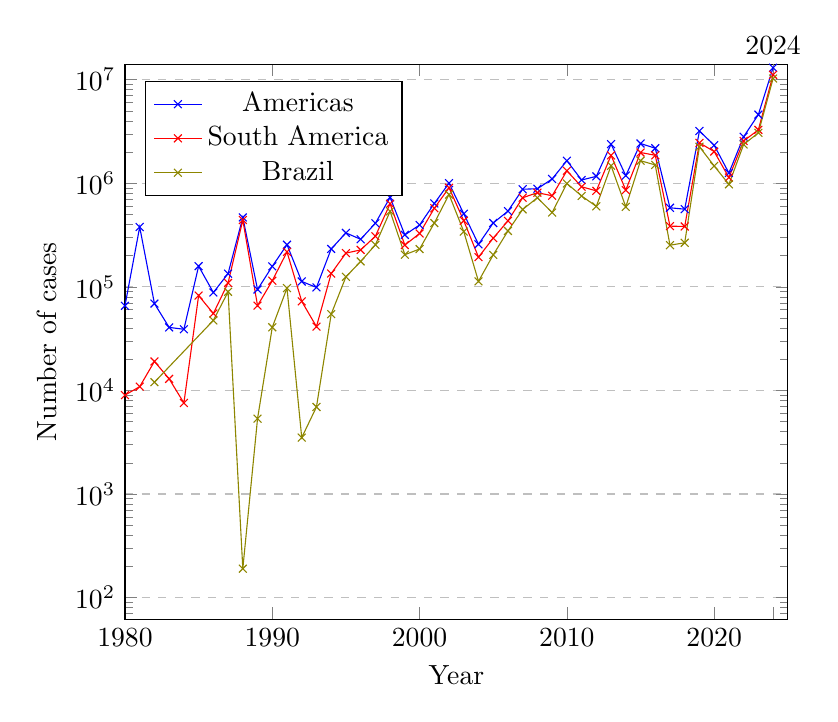
\begin{tikzpicture}[>=latex, scale=1]
		%scale=.6]
		\begin{axis}[
				width = {10cm},
				%title={Dengue reported cases from 1980 to 2022},
				xlabel={Year},
				ylabel={Number of cases},
				ymode=log,
				xmin=1980, xmax=2025,
				ymin=0, ymax=14000000,
				xtick={1980, 1990, 2000, 2010, 2020, 2024},
				xticklabels={1980, 1990, 2000, 2010, 2020},
				extra x ticks={2024},
				extra x tick labels={2024},  % Labels at top
				extra x tick style={ticklabel pos=upper},
				legend pos=north west,
				ymajorgrids=true,
				grid style=dashed,
			]

			\addplot[
				color=blue,
				mark=x,
			]
			plot coordinates {
					(1980, 65523)
					(1981, 377916)
					(1982, 68892)
					(1983, 40544)
					(1984, 38904)
					(1985, 158193)
					(1986, 88093)
					(1987, 134013)
					(1988, 467386)
					(1989, 94179)
					(1990, 157662)
					(1991, 254749)
					(1992, 112567)
					(1993, 98598)
					(1994, 232051)
					(1995, 331417)
					(1996, 287519)
					(1997, 410392)
					(1998, 729425)
					(1999, 317158)
					(2000, 394857)
					(2001, 636977)
					(2002, 1001073)
					(2003, 506726)
					(2004, 257251)
					(2005, 413122)
					(2006, 537412)
					(2007, 874750)
					(2008, 884334)
					(2009, 1099742)
					(2010, 1648569)
					(2011, 1073990)
					(2012, 1164366)
					(2013, 2384803)
					(2014, 1184045)
					(2015, 2416018)
					(2016, 2175409)
					(2017, 579027)
					(2018, 561689)
					(2019, 3190778)
					(2020, 2326115)
					(2021, 1254648)
					(2022, 2811433)
					(2023, 4594823)
					(2024, 13036652)
				};
			\addlegendentry{Americas}

			\addplot[
				color=red,
				mark=x,
			]
			plot coordinates {
					(1980, 9003)
					(1981, 10861)
					(1982, 19034)
					(1983, 12925)
					(1984, 7560)
					(1985, 82273)
					(1986, 55248)
					(1987, 108955)
					(1988, 441382)
					(1989, 65803)
					(1990, 114431)
					(1991, 217077)
					(1992, 72319)
					(1993, 41250)
					(1994, 134342)
					(1995, 211396)
					(1996, 226960)
					(1997, 307625)
					(1998, 632804)
					(1999, 252762)
					(2000, 326846)
					(2001, 572876)
					(2002, 903891)
					(2003, 434264)
					(2004, 193334)
					(2005, 294943)
					(2006, 432661)
					(2007, 724077)
					(2008, 810134)
					(2009, 756755)
					(2010, 1317801)
					(2011, 923793)
					(2012, 843840)
					(2013, 1857228)
					(2014, 857983)
					(2015, 1978921)
					(2016, 1860466)
					(2017, 385076)
					(2018, 382243)
					(2019, 2453060)
					(2020, 2021272)
					(2021, 1134555)
					(2022, 2558083)
					(2023, 3274879)
					(2024, 11118085)
				};
			\addlegendentry{South America}

			\addplot[
				color=olive,
				mark=x,
			]
			plot coordinates {
					(1980, 0)
					(1981, 0)
					(1982, 12000)
					(1983, 0)
					(1984, 0)
					(1985, 0)
					(1986, 47367)
					(1987, 89393)
					(1988, 190)
					(1989, 5334)
					(1990, 40642)
					(1991, 97209)
					(1992, 3501)
					(1993, 6915)
					(1994, 54453)
					(1995, 124775)
					(1996, 175749)
					(1997, 254074)
					(1998, 535283)
					(1999, 204131)
					(2000, 231412)
					(2001, 412388)
					(2002, 778037)
					(2003, 341189)
					(2004, 112851)
					(2005, 203356)
					(2006, 345922)
					(2007, 558413)
					(2008, 724427)
					(2009, 520660)
					(2010, 994158)
					(2011, 753487)
					(2012, 597450)
					(2013, 1473645)
					(2014, 591080)
					(2015, 1649008)
					(2016, 1500535)
					(2017, 252054)
					(2018, 265934)
					(2019, 2248570)
					(2020, 1467142)
					(2021, 975474)
					(2022, 2363490)
					(2023, 3064739)
					(2024, 10239883)
				};
			\addlegendentry{Brazil}
		\end{axis}
	\end{tikzpicture}
	\caption{Dengue reported cases from 1980 to 2024~\citep{paho-1}.}
	\label{fig:dengue_reported_cases_graphic}
\end{figure}

The disease imposes substantial social and economic burdens, affecting not only
the health and well-being of individuals but also the broader economic
productivity and healthcare system. The financial impact of Dengue in Brazil is
profound, for example, annual expenditures on Dengue prevention and control
exceed BRL $1.6$ billion~\citep{negreiros-2020}. The direct costs include
healthcare expenses for hospitalization, medical treatment, and public health
campaigns aimed at controlling mosquito populations~\citep{negreiros:2008}.
Indirect costs, such as lost productivity due to illness and the long-term
effects of severe Dengue cases, add to the financial strain. Moreover, the
social consequences are equally alarming, with communities enduring the
disruption of daily life, increased anxiety over disease outbreaks, and the loss
of lives.

Despite the severity of the situation, most Brazilian municipalities continue to
make crucial decisions in combating Dengue without the support of advanced
computational tools~\citep{brasil-dept-helth:2009}. The current approach is
largely reactive, relying on traditional mosquito control methods, including
eliminating adult mosquitoes, their breeding sites and public health
interventions. These actions are often insufficient to address the complexity
and scale of the problem. This lack of computational support means that
decisions regarding resource allocation, strategic planning, and the deployment
of interventions are not optimized, leading to possible inefficiencies and
potentially exacerbating the spread of the
disease~\citep{forbes-2002,xie-2015,rais-2011}.

The most common approach to combating Dengue spread is employing chemical
control methods, such as insecticides, which manage the mosquito population in
both the larval and adult stages~\citep{brasil-dept-helth:2009}. The \gls{who}
provides technical and operational standards for pesticide experts to ensure the
safe use of insecticides in public health. These standards specify the active
ingredients and dosages for various treatments. During disease outbreaks,
emergency responses in urban areas usually involve the dispatch of spraying
vehicles to apply insecticides (see Figure~\ref{fig:nebulizer}). It is essential
to use insecticides carefully and responsibly in vector control activities, as
indiscriminate use can have significant environmental impacts and contribute to
developing resistance in mosquitoes~\citep{WHO2009,WHO2020}.

\begin{figure}[h!]
	\centering
	\includegraphics[scale=0.5]{images/fumace.jpg}
	\caption{Nebulizer equipment attached to vehicle \citep{fumace-2022}.}
	\label{fig:nebulizer}
\end{figure}

The sprayed insecticide has no residual  effect and it is strongly influenced by
wind  and obstacles  along the  streets. The  best effect  is achieved  when the
densest  insecticide cloud  is at  a distance  of at  most 100  meters from  the
equipment~\citep{brasil-dept-helth:2009}.  As this  distance  is  crossed, the
effectiveness  decreases, as a consequence of droplet drift influenced by
factors of the environment. The cloud dispersion is illustrated in
Figure~\ref{fig:dispersion}.

\begin{figure}[!ht]
	\centering
	\includegraphics[scale=0.4]{images/cloud-dispersion.png}
	\caption{Cloud dispersion of the application \citep{brasil-dept-helth:2009}.}
	\label{fig:dispersion}
\end{figure}

Insecticide application instructions are generally based on ideal topology
conditions, locality structure, and favorable winds. The operation is often
affected by unpaved roads, the presence of high walls,  and  high   vegetation,
in  addition  to   headwinds.  The application methodology must consider these
limitations to obtain a good impact on the vector population. Once a spraying
vehicle begins to service a city block, it must sequentially cover all
surrounding streets in a clockwise direction. The traversal ensures that the
insecticide fog forms a continuous barrier, preventing mosquitoes from escaping.
The clockwise direction is due to real operational factors, as the nebulizer
equipment points to the right side of the vehicle.

Figure~\ref{fig:instance_digraph_fumace_car} shows an example of a map, with
four blocks to service, and Figure~\ref{fig:route_fumace_car} presents a
spraying route for these blocks where the nebulizer is activated in the black
dots and follows the direction of the arrow, starts by serving Block 2, goes to
Blocks 1, 3 and 4, respectively.

\begin{figure}[!ht]
	\begin{minipage}[c]{.49\textwidth}
		\centering
		\subfloat[Street blocks example.]{\label{fig:instance_digraph_fumace_car}\includegraphics[width=5cm, height=5cm]{images/cbrp-instance.pdf}} \end{minipage}%
	\begin{minipage}[c]{.49\textwidth}
		\centering
		\subfloat[Spraying route example.]{\label{fig:route_fumace_car}\includegraphics[width=8cm, height=5cm]{images/nebulizer-activated.pdf}}
	\end{minipage}
	\caption{Vehicle pattern with nebulizer \cite{brasil-dept-helth:2009}.}
\end{figure}

As a result, health authorities with limited budgets must make two key
decisions: first, selecting which city blocks should receive insecticide
spraying to maximize vector suppression; and second, optimizing vehicle routes
to ensure the efficient use of available resources. In this context, there is a
clear and urgent need to integrate computational models and decision-support
systems into Dengue control strategies. Such tools can help municipalities
better predict outbreaks, optimize resource use, and implement more effective
mosquito control measures.

In operations research, routing problems are typically classified based on where
the service is performed. When services are provided at specific locations
(nodes), they fall under \gls{vrp}~\citep{braekers2016vehicle}. When services
are conducted along edges (or arcs), they are categorized as
\gls{arp}~\citep{corberan2021arc}. The routing challenge in Dengue control
exhibits the characteristics of both \gls{vrp} and \gls{arp}. Each city block
can be represented as a \textit{super-node} (similar to a \gls{vrp}), while
spraying occurs along the surrounding arcs, aligning with \gls{arp} features.
Given this hybrid structure, we introduce and explore a new problem, titled the
\gls{cbrp}.

The \gls{cbrp} aims to optimize the servicing of city blocks within an urban
street network by assigning spraying vehicles. However, due to limited
operational resources, only a subset of city blocks can be serviced. A city
block is considered serviced if a spraying vehicle completely encircles it
without detours, and each serviced block contributes a predefined benefit. Thus,
the primary objective of the \gls{cbrp} is to identify the subset of blocks
whose servicing yields the highest aggregate benefit, alongside determining the
optimal vehicle routes to achieve this objective within the available resources.

The Figure~\ref{fig:ex1} illustrates an example of an input graph (city map) and
a corresponding \gls{cbrp} feasible solution. In Figure~\ref{subfig:a}, the
circles represent the graph nodes, while the labels from A to H indicate the
city blocks. Figure~\ref{subfig:b} depicts a feasible solution to the
\gls{cbrp}. In this solution, the nodes used in the route are marked as squares
and connected by black arrows (nodes 4, 5, 3, and 9). Squares with a double
border denote nodes that act as starting points to serve at least one block. The
atended blocks are represented by the arcs connected to the double square with
the same color, for example: node 4 (blue) serves blocks A (arcs
4$\rightarrow$8, 8$\rightarrow$1 and 1$\rightarrow$4) and B (arcs
4$\rightarrow$6, 6$\rightarrow$8 and 8$\rightarrow$4). Node 5 (red) serves
blocks D and F, node 3 does not serve any block, and node 9 (teal) serves block
H.

\begin{figure}[!ht]
	\begin{subfigure}{.5\textwidth}
		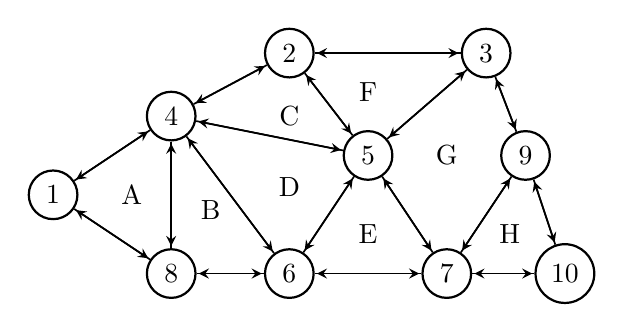
\begin{tikzpicture}[
				> = stealth, % arrow head style
				shorten > = 0.8pt, % don't touch arrow head to node
				auto,
				node distance = 1cm, % distance between nodes
				semithick % line style
			]

			\tikzstyle{every state}=[
			draw = black,
			thick,
			fill = white,
			minimum size = 5mm
			]

			\node[state] (a) [at={(-1, -0.5)}]{$1$};
			\node[state] (b) [at={(2,1.3)}] {$2$};
			\node[state] (c) [at={(4.5,1.3)}] {$3$};
			\node[state] (d) [at={(0.5, 0.5)}] {$4$};
			\node[state] (e) [at={(3, 0)}] {$5$};
			\node[state] (f) [at={(2,-1.5)}] {$6$};
			\node[state] (g) [at={(4,-1.5)}] {$7$};
			\node[state] (i) [at={(0.5,-1.5)}] {$8$};
			\node[state] (j) [at={(5,0)}] {$9$};
			\node[state] (k) [at={(5.5,-1.5)}] {$10$};
			% Blocks
			\node[state, draw = white, right of = a] {A};
			\node[state, draw = white, right of = i, yshift=0.8cm, xshift=-0.5cm] {B};
			\node[state, draw = white, below of = b, yshift=0.2cm] {C};
			\node[state, draw = white, left of = e, yshift=-0.4cm] {D};
			\node[state, draw = white, below of = e] {E};
			\node[state, draw = white, right of = b, yshift=-0.5cm] {F};
			\node[state, draw = white, right of = e] {G};
			\node[state, draw = white, below of = j, xshift=-0.2cm] {H};


			\path[->] (a) edge node {} (d);
			\path[->] (d) edge node {} (a);
			\path[->] (i) edge node {} (a);
			\path[->] (a) edge node {} (i);
			\path[->] (b) edge node {} (d);
			\path[->] (d) edge node {} (b);
			\path[->] (b) edge node {} (c);
			\path[->] (c) edge node {} (b);
			\path[->] (c) edge node {} (e);
			\path[->] (e) edge node {} (c);
			\path[->] (e) edge node {} (f);
			\path[->] (f) edge node {} (e);
			\path[->] (d) edge node {} (i);
			\path[->] (i) edge node {} (d);
			\path[->] (d) edge node {} (e);
			\path[->] (e) edge node {} (d);
			\path[->] (d) edge node {} (f);
			\path[->] (f) edge node {} (d);
			\path[->] (e) edge node {} (g);
			\path[->] (g) edge node {} (e);
			\path[->] (c) edge node {} (j);
			\path[->] (j) edge node {} (c);
			\path[->] (i) edge node {} (f);
			\path[->] (f) edge node {} (i);
			\path[->] (j) edge node {} (k);
			\path[->] (k) edge node {} (j);
			\path[->] (j) edge node {} (g);
			\path[->] (g) edge node {} (j);
			\path[->] (e) edge node {} (b);
			\path[->] (b) edge node {} (e);
			\path[->] (f) edge node {} (g);
			\path[->] (g) edge node {} (f);
			\path[->] (g) edge node {} (k);
			\path[->] (k) edge node {} (g);

		\end{tikzpicture}
		\subcaption{\label{subfig:a} Initial graph and blocks.}
	\end{subfigure}
	% Segunda figura
	\begin{subfigure}{.5\textwidth}
		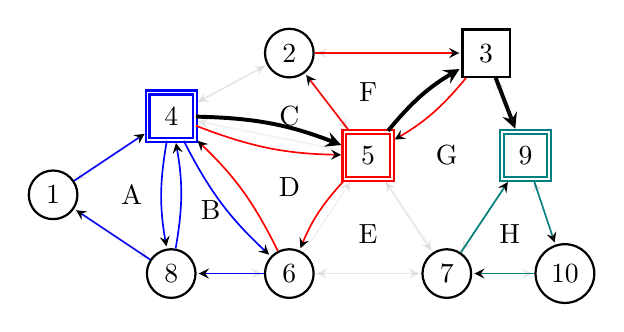
\begin{tikzpicture}[
				> = stealth, % arrow head style
				shorten > = 0.8pt, % don't touch arrow head to node
				auto,
				node distance = 1cm, % distance between nodes
				semithick % line style
			]

			\tikzstyle{every state}=[
			draw = black,
			thick,
			fill = white,
			minimum size = 6mm
			]

			\node[state] (a) [at={(-1, -0.5)}]{$1$};
			\node[state] (b) [at={(2,1.3)}] {$2$};
			\node[state, rectangle] (c) [at={(4.5,1.3)}] {$3$};
			\node[state, rectangle, double, draw=blue] (d) [at={(0.5, 0.5)}] {$4$};
			\node[state, rectangle, double, draw=red] (e) [at={(3, 0)}] {$5$};
			\node[state] (f) [at={(2,-1.5)}] {$6$};
			\node[state] (g) [at={(4,-1.5)}] {$7$};
			\node[state] (i) [at={(0.5,-1.5)}] {$8$};
			\node[state, rectangle, double, draw=teal] (j) [at={(5,0)}] {$9$};
			\node[state] (k) [at={(5.5,-1.5)}] {$10$};
			% Blocks
			\node[state, thick, dashed, draw = white, right of = a] {A};
			\node[state, thick, dashed, draw = white, right of = i, yshift=0.8cm, xshift=-0.5cm] {B};
			\node[state, draw = white, below of = b, yshift=0.2cm] {C};
			\node[state, thick, dashed, draw = white, left of = e, yshift=-0.4cm] {D};
			\node[state, draw = white, below of = e] {E};
			\node[state, thick, dashed, draw = white, right of = b, yshift=-0.5cm] {F};
			\node[state, draw = white, right of = e] {G};
			\node[state, thick, dashed, draw = white, below of = j, xshift=-0.2cm] {H};
			% Dummy
			%\node[state, double, above of = a] (s) {s};
			%\node[state, double, right of = j, xshift=0.2cm] (t) {t};
			%\path[->, draw = black, opacity = 1.0] (s) edge node {} (d);
			%\path[->, draw = black, opacity = 1.0] (j) edge node {} (t);

			\path[->, draw = blue, opacity = 1.0] (a) edge node {} (d);
			\path[->, draw = gray, opacity = 0.1] (d) edge node {} (a);
			\path[->, draw = blue, opacity = 1.0] (i) edge node {} (a);
			\path[->, draw = gray, opacity = 0.1] (a) edge node {} (i);
			\path[->, draw = gray, opacity = 0.1] (b) edge node {} (d);
			\path[->, draw = gray, opacity = 0.1] (d) edge node {} (b);
			\path[->, draw = red, opacity = 1.0] (b) edge node {} (c);
			\path[->, draw = gray, opacity = 0.1] (c) edge node {} (b);
			\path[->, draw = red, opacity = 1.0, bend left=10] (c) edge node {} (e);
			\path[->, draw = black, opacity = 1.0, bend left=10, line width=0.5mm] (e) edge node {} (c);
			\path[->, draw = red, opacity = 1.0, bend right=10] (e) edge node {} (f);
			\path[->, draw = gray, opacity = 0.1] (f) edge node {} (e);
			\path[->, draw = blue, opacity = 1.0, bend right=10] (d) edge node {} (i);
			\path[->, draw = blue, opacity = 1.0, bend right=10] (i) edge node {} (d);
			\path[->, draw = black, opacity = 1.0, bend left=10, line width=0.5mm] (d) edge node {} (e);
			\path[->, draw = red, opacity = 1.0, bend right=10] (d) edge node {} (e);
			\path[->, draw = gray, opacity = 0.1] (e) edge node {} (d);
			\path[->, draw = blue, opacity = 1.0, bend right=10] (d) edge node {} (f);
			\path[->, draw = red, opacity = 1.0, bend right=10] (f) edge node {} (d);
			\path[->, draw = gray, opacity = 0.1] (e) edge node {} (g);
			\path[->, draw = gray, opacity = 0.1] (g) edge node {} (e);
			\path[->, draw = black, opacity = 1.0, line width=0.5mm] (c) edge node {} (j);
			\path[->, draw = gray, opacity = 0.1] (j) edge node {} (c);
			\path[->, draw = gray, opacity = 0.1] (i) edge node {} (f);
			\path[->, draw = blue, opacity = 1.0] (f) edge node {} (i);
			\path[->, draw = teal, opacity = 1.0] (j) edge node {} (k);
			\path[->, draw = gray, opacity = 0.1] (k) edge node {} (j);
			\path[->, draw = gray, opacity = 0.1] (j) edge node {} (g);
			\path[->, draw = gray, opacity = 0.1] (g) edge node {} (j);
			\path[->, draw = red, opacity = 1.0] (e) edge node {} (b);
			\path[->, draw = gray, opacity = 0.1] (b) edge node {} (e);
			\path[->, draw = gray, opacity = 0.1] (f) edge node {} (g);
			\path[->, draw = gray, opacity = 0.1] (g) edge node {} (f);
			\path[->, draw = gray, opacity = 0.1] (g) edge node {} (k);
			\path[->, draw = teal, opacity = 1.0] (k) edge node {} (g);
			\path[->, draw = teal, opacity = 1.0] (g) edge node {} (j);
		\end{tikzpicture}
		\subcaption{\label{subfig:b} Route and attended blocks.}
	\end{subfigure}
	\caption{\label{fig:ex1} CBRP instance (a) and solution (b).}
\end{figure}

Given the complex and dynamic nature of urban environments, particularly in
public health scenarios like Dengue control, incorporating stochastic elements
into the \gls{cbrp} is essential to enhance the realism and applicability of the
solution. Some unpredictable behavior of mosquitoes and the spread of Dengue
cases during seasons of the years highlight the need for a stochastic version of
the \gls{cbrp}. This leads to solutions that better reflect the variability of
actual deployment scenarios, improving the adherence of the model to real-world
challenges. Moreover, by accounting for probabilistic factors, stochastic
approaches can prioritize the most critical city blocks under uncertain resource
availability, thereby increasing the effectiveness and resilience of vector
control interventions.

The \gls{cbrp} extends beyond its application in vector control, providing a
robust framework to address a variety of urban logistics challenges. These
challenges include waste collection, postal delivery, and reading of utility
meters, where the primary goal is to efficiently service city blocks while
managing both spatial and resource constraints. The flexibility of the
\gls{cbrp} makes it particularly valuable in densely populated urban
environments, where the efficiency of routing decisions significantly affects
both service effectiveness and operational costs.

Besides the definition of control actions~\citep{gomez-2009,jing2019dengue}, it
is important to develop visualization and decision support tools to assist the
health departments. A clear understanding of the likely progression of Dengue
cases can significantly enhance short-term resource allocation
strategies~\citep{brasil-dept-helth:2009}. Generating accurate predictive models
for Dengue spread, especially in urban areas is highly challenging since
mosquito behavior is inconsistent and depends on numerous factors. These include
the availability and location of breeding sites, the mosquito population size
and infection rate, the timing and location of insecticide application,
frequency of rainfall, various climate conditions, and the interactions between
mosquitoes, breeding sites, and human populations.

In this thesis, we developed a complete set of methodologies focused in the
application of \gls{cbrp} to optimize insecticide-spraying routes for Dengue
control. Those methodologies compreend exact and heuristic approaches for
deterministic and stochastic versions of the \gls{cbrp}, instances based on real
data, robust simulation based on multi-agent systems and a
simulation-optimization framework that could assist health departments. This
application is particularly pertinent to many Brazilian cities, where seasonal
outbreaks of mosquito-borne diseases demand resource-efficient, targeted vector
control strategies. By optimizing spray routes, the \gls{cbrp} not only improves
operational efficiency but also maximizes coverage of high-risk areas,
ultimately supporting public health initiatives aimed at reducing Dengue
transmission.

% The \gls{mabs} have become increasingly popular in various fields due to their
% ability to capture the complexity and dynamics of real-world
% systems~\citep{siebers-2008}. Unlike traditional simulations that rely on a set
% of predetermined rules and assumptions, multi-agent simulations allow for
% interactions between agents to emerge organically, leading to the emergence of
% unexpected and emergent behaviors. This makes them an effective tool for
% understanding and predicting the behavior of complex systems, such as social and
% economic systems, ecological systems, and even biological
% systems~\citep{ballet-2020}. Additionally, multi-agent simulations provide a
% flexible and adaptable approach that can be easily modified and scaled to
% simulate different scenarios and environments. With the increasing availability
% of computing resources, multi-agent simulations have become an important tool
% for modeling and simulating complex systems, providing valuable insights into
% the behavior and evolution of these systems~\citep{selvaratnam-1995}.


%\paragraph{Our contributions.} The contributions of this study are three-fold.
% First, it advances vector control strategies by proposing novel methodologies
% for the optimal routing of spraying vehicles. Our approaches are based on
% mixed-integer linear programming (MILP) formulations and biased-random key
% genetic algorithms (BRKGA). Second, we introduce a systematic procedure for
% generating realistic problem instances by mapping city blocks and their
% surrounding street arcs. Third, through extensive computational experiments
% utilizing seven years of Dengue case data from two Brazilian cities, we
% demonstrate that our proposed methodologies significantly improve vector
% control effectiveness, potentially reducing Dengue transmission rates and
% improving public health outcomes. These findings offer valuable insights to
% public health authorities, policymakers, and researchers working on complex
% vector-borne disease challenges. Moreover, the generality of the CBRP
% framework makes it a promising approach for optimizing vehicle routing
% strategies in other city-block service applications.

% \paragraph{Text organization.}
% The remainder of this thesis is organized as follows.
% Chapter~\ref{chp:preliminary-concepts} formally defines the City Block Routing Problem (CBRP).
% Chapter~\ref{chp:literature_review} reviews existing operations research, \gls{ml} and simulation approaches relevant to Dengue vector control.
% Section~\ref{sec:models} introduces and describes the proposed mathematical formulations for the CBRP.
% Section~\ref{sec:data} explains the datasets and experimental setups employed to evaluate the proposed methodologies.
% Section~\ref{sec:results} discusses computational results and assesses the methodologies' performance.
% Finally, Section~\ref{sec:conclusions} summarizes the findings and provides concluding remarks.
\chapter{Preliminary Concepts and Formulations}\label{chp:preliminary-concepts}

In this chapter, we introduce the fundamental concepts necessary for
understanding this thesis. The basic notation and definitions are presented in
Section~\ref{sec:not-e-def}. In this work, we employ basic concepts from
Combinatorial Optimization, which are assumed to be known. If the reader deems a
review necessary, we recommend the textbook by Nemhauser and
Wolsey~\cite{Nemhauser}, which covers this topic with a focus on \gls{ilp}, one
of the main tools used in this work. Basic concepts related to graph theory are
also assumed to be known. Should the
reader require a refresher, the material can be found in standard textbooks on
the subject, such as Diestel~\cite{diestel:2005}. 

% TODO: add references to the sections
% The mathematical models are presented in Sections~\ref{sec:dmfm-pma}
% and~\ref{sec:ab-pma}. Section~\ref{sec:rel-lagrangiana} provides a description
% of the functioning and application of Lagrangian relaxation, one of the main
% approaches employed in this work. Finally, in Sections~\ref{sec:metaheuristic}
% and~\ref{subsec:brkga}, we present a general discussion on metaheuristics.


\section{Notations and Definitions}\label{sec:not-e-def}

Once a spraying vehicle begins to service a city block, it must sequentially
cover all surrounding edges in a clockwise direction. The
traversal ensures that the insecticide fog forms a continuous barrier,
preventing mosquitoes from escaping. 
The clockwise direction is due to real operational factors, 
as the nebulizer equipment points to the right side of the
vehicle. 
Figure~\ref{fig:instance_digraph_fumace_car} shows an example of a map,
with four blocks to service, and Figure~\ref{fig:route_fumace_car} presents a
spraying route for these blocks where the nebulizer is activated in the black
dots and follows the direction of the arrow, starts by serving Block 2, goes to
Blocks 1, 3 and 4, respectively. 

\begin{figure}[!ht]
	\begin{minipage}[c]{.49\textwidth}
		\centering
		\subfloat[A CBRP instance
			digraph.]{\label{fig:instance_digraph_fumace_car}\includegraphics[width=5cm,
				height=5cm]{images/cbrp-instance.pdf}} \end{minipage}%
	\begin{minipage}[c]{.49\textwidth}
		\centering
		\subfloat[A spraying vehicle route covering four city
			blocks.]{\label{fig:route_fumace_car}\includegraphics[width=8cm,
				height=5cm]{images/nebulizer-activated.pdf}}
	\end{minipage}
	\caption{\label{fig:route-ex} CBRP example.}
\end{figure}


Let $G = (V, A, B)$ be a weighted and directed graph, where $V = \{1, \dots, n\}$
is the set of vertices, $A = \{(i, j) : i, j \in V, i \neq j\}$
is the set of $m$ arcs, and $B = \{b : b \subseteq V\}$ is the set of blocks.
In each arc, the first vertex is the source and also the
predecessor of the second vertex in the ordered pair, which is known as the
destination. Each block $b$ has an associated set of arcs $B(i, j) \subseteq A$ that
can be serviced by a vehicle. 

We now present a formal definition of the \gls{cbrp}. Let a Plannar Graph,
extracted from a real citymap, be represented as a weighted directed graph
$G$. Each node in $V$ represents the intersection of at least two
streets and has a list of blocks $b \subseteq B$ that are associated with it.
Each arc $(i, j) \in A$ has a deadheading time $t_{i, j} > 0$, a service time
$t^{'}_{i, j} > 0$ such that $t_{i, j} \leqslant t^{'}_{i, j}$ and the block
$b \in B$ that is associated with it. The input to the \gls{cbrp} is defined as:

\begin{itemize}
	\item $G = (V, A, B)$ is a weighted directed planar graph with the blocks associated with it;
	\item $p_b : B \rightarrow \mathbb{N}$ is a function that returns the profit
	      for each block $b \in B$;
	\item $t_{i, j} : A \rightarrow \mathbb{N}$ is a function that returns the
	      deadheading time for each arc $(i, j) \in A$;
	\item $t^{'}_{i, j} : A \rightarrow \mathbb{N}$ is a function that returns
	      the service time for each arc $(i, j) \in A$;
	\item $T$ is the time limit for the vehicle to travel and service the blocks;
	\item $V(b)$ is the set of nodes that are associated with the block $b \in B$;
	\item $B(i)$ is the set of blocks that are associated with the node $i \in V$;
	\item $B(i, j)$ is the set of blocks that are associated with the arc $(i, j) \in A$;
	\item $\delta^{+}_{i}$ is the set of arcs with destination $i$;
	\item $\delta^{-}_{i}$ is the set of arcs with source $i$;
\end{itemize}

The \gls{cbrp} is introduced as a general framework for addressing the routing of
spraying vehicles and other city block servicing problems. 
The objective of the \gls{cbrp} is to determine an optimal traversal that 
services a subset of blocks within a network, maximizing the total 
collected benefit from each serviced block. 
A vehicle traverses the graph $G$ following a route that can serve a
subset of blocks within a given time limit $T$. This work considers two types of 
solution routes, depending on whether the vertices can be
visited more than once: \textit{Walk-based route}, in which any vertex (or arc)
can be visited multiple times and \textit{Path-based route}, in which no vertex
appears more than once. 
An optimal route (walk or path) is one that maximizes
the total prize collected from the serviced blocks while respecting the vehicle
time limit $T$.

To facilitate modeling, we augment the graph $G$ by introducing a dummy depot
$0$, from which the route originates, and a set of arcs $\{(0, i), (i, 0) :
	\forall i \in V\}$ with times $t_{i,0} = t_{0,i} = 0$, $\forall i \in V$. 
Thus, we define the modified graph as $G' = (V' = V \cup \{0\}, A' = A \cup \{(0,
	i), (i, 0) : \forall i \in V\})$.

We now present key properties of the \gls{cbrp}. First, due to the operational
restrictions, once a block $b$ starts being serviced at a given node $i$, it
must be fully encircled before the vehicle moves to another block. This leads
to the following property:

\begin{property}
	\label{claim:core_insight}
	A block can be serviced if at least one of its nodes is visited.
\end{property}

From Property~\ref{claim:core_insight}, 
when formulating the problem, it is not
necessary to explicitly require the vehicle to completely traverse a block's
perimeter in order to count it as serviced. Instead, servicing can be achieved
by visiting at least one node within the block and accounting for the
corresponding service time. This property is valid due to the definition of the blocks $B$ and
the fact that the vehicle must service all blocks in a clockwise direction.

Figure~\ref{fig:servicing_block_no_surrounding_strategy} illustrates an example of
this strategy, where servicing is achieved without requiring a full traversal of
the block's perimeter.

\begin{figure}[!ht]
	\begin{minipage}[c]{.32\textwidth}
		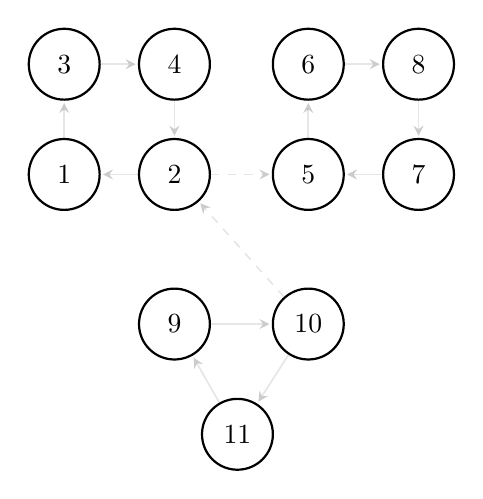
\begin{tikzpicture}[
				> = stealth, % arrow head style
				shorten > = 0.8pt, % don't touch arrow head to node
				auto,
				node distance = 1.4cm, % distance between nodes
				semithick % line style
			]
			
			\tikzstyle{every state}=[
			draw = black,
			thick,
			fill = white,
			minimum size = 9mm
			]
			
			\node[state] (a) at (0,0) {$1$};
			\node[state, right of = a] (b) {$2$};
			\node[state, above of = a] (c) {$3$};
			\node[state, above of = b] (d) {$4$};
			
			\node[state, right of = b, xshift=0.3cm] (e) {$5$};
			\node[state, right of = d, xshift=0.3cm] (f) {$6$};
			\node[state, right of = e] (g) {$7$};
			\node[state, right of = f] (h) {$8$};
			
			\node[state, below of = b, yshift=-0.5cm] (i) {$9$};
			\node[state, below of = e, yshift=-0.5cm] (j) {$10$};
			\node[state, below of = i, left of = j, xshift=0.5cm] (k) {$11$};
			
			\path[->, draw = gray, opacity = 0.2] (a) edge node {} (c); 
			\path[->, draw = gray, opacity = 0.2] (c) edge node {} (d); 
			\path[->, draw = gray, opacity = 0.2] (d) edge node {} (b);
			\path[->, draw = gray, opacity = 0.2] (b) edge node {} (a);
			
			\path[->, draw = gray, opacity = 0.2] (e) edge node {} (f);
			\path[->, draw = gray, opacity = 0.2] (f) edge node {} (h);
			\path[->, draw = gray, opacity = 0.2] (h) edge node {} (g);
			\path[->, draw = gray, opacity = 0.2] (g) edge node {} (e);
			
			\path[->, draw = gray, opacity = 0.2] (i) edge node {} (j);
			\path[->, draw = gray, opacity = 0.2] (j) edge node {} (k);
			\path[->, draw = gray, opacity = 0.2] (k) edge node {} (i);
			
			\path[->, draw = gray, opacity = 0.2, dashed] (j) edge node {} (b);
			\path[->, draw = gray, opacity = 0.2, dashed] (b) edge node {} (e);
		\end{tikzpicture}
		\subcaption{Instance Example.}
	\end{minipage}
	\hfill
	\begin{minipage}[c]{.32\textwidth}
		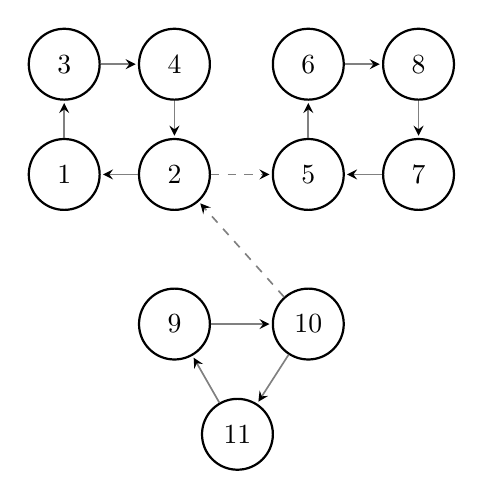
\begin{tikzpicture}[
				> = stealth, % arrow head style
				shorten > = 0.8pt, % don't touch arrow head to node
				auto,
				node distance = 1.4cm, % distance between nodes
				semithick % line style
			]
			
			\tikzstyle{every state}=[
			draw = black,
			thick,
			fill = white,
			minimum size = 9mm
			]
			
			\node[state] (a) at (0,0) {$1$};
			\node[state, right of = a] (b) {$2$};
			\node[state, above of = a] (c) {$3$};
			\node[state, above of = b] (d) {$4$};
			
			\node[state, right of = b, xshift=0.3cm] (e) {$5$};
			\node[state, right of = d, xshift=0.3cm] (f) {$6$};
			\node[state, right of = e] (g) {$7$};
			\node[state, right of = f] (h) {$8$};
			
			\node[state, below of = b, yshift=-0.5cm] (i) {$9$};
			\node[state, below of = e, yshift=-0.5cm] (j) {$10$};
			\node[state, below of = i, left of = j, xshift=0.5cm] (k) {$11$};
			
			\path[->, draw = gray, opacity = 1.0] (a) edge node {} (c); 
			\path[->, draw = gray, opacity = 1.0] (c) edge node {} (d); 
			\path[->, draw = gray, opacity = 1.0] (d) edge node {} (b);
			\path[->, draw = gray, opacity = 1.0] (b) edge node {} (a);
			
			\path[->, draw = gray, opacity = 1.0] (e) edge node {} (f);
			\path[->, draw = gray, opacity = 1.0] (f) edge node {} (h);
			\path[->, draw = gray, opacity = 1.0] (h) edge node {} (g);
			\path[->, draw = gray, opacity = 1.0] (g) edge node {} (e);
			
			\path[->, draw = gray, opacity = 1.0] (i) edge node {} (j);
			\path[->, draw = gray, opacity = 1.0] (j) edge node {} (k);
			\path[->, draw = gray, opacity = 1.0] (k) edge node {} (i);
			
			\path[->, draw = gray, opacity = 1.0, dashed] (j) edge node {} (b);
			\path[->, draw = gray, opacity = 1.0, dashed] (b) edge node {} (e);
		\end{tikzpicture}
		\subcaption{Explicity Block Servicing.}
	\end{minipage}\\
	\centering
	\begin{minipage}[c]{.32\textwidth}
		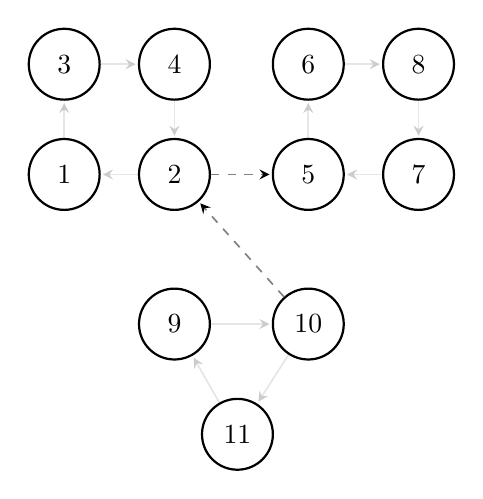
\begin{tikzpicture}[
				> = stealth, % arrow head style
				shorten > = 0.8pt, % don't touch arrow head to node
				auto,
				node distance = 1.4cm, % distance between nodes
				semithick % line style
			]
			
			\tikzstyle{every state}=[
			draw = black,
			thick,
			fill = white,
			minimum size = 9mm
			]
			
			\node[state] (a) at (0,0) {$1$};
			\node[state, right of = a] (b) {$2$};
			\node[state, above of = a] (c) {$3$};
			\node[state, above of = b] (d) {$4$};
			
			\node[state, right of = b, xshift=0.3cm] (e) {$5$};
			\node[state, right of = d, xshift=0.3cm] (f) {$6$};
			\node[state, right of = e] (g) {$7$};
			\node[state, right of = f] (h) {$8$};
			
			\node[state, below of = b, yshift=-0.5cm] (i) {$9$};
			\node[state, below of = e, yshift=-0.5cm] (j) {$10$};
			\node[state, below of = i, left of = j, xshift=0.5cm] (k) {$11$};
			
			\path[->, draw = gray, opacity = 0.2] (a) edge node {} (c); 
			\path[->, draw = gray, opacity = 0.2] (c) edge node {} (d); 
			\path[->, draw = gray, opacity = 0.2] (d) edge node {} (b);
			\path[->, draw = gray, opacity = 0.2] (b) edge node {} (a);
			
			\path[->, draw = gray, opacity = 0.2] (e) edge node {} (f);
			\path[->, draw = gray, opacity = 0.2] (f) edge node {} (h);
			\path[->, draw = gray, opacity = 0.2] (h) edge node {} (g);
			\path[->, draw = gray, opacity = 0.2] (g) edge node {} (e);
			
			\path[->, draw = gray, opacity = 0.2] (i) edge node {} (j);
			\path[->, draw = gray, opacity = 0.2] (j) edge node {} (k);
			\path[->, draw = gray, opacity = 0.2] (k) edge node {} (i);
			
			\path[->, draw = gray, opacity = 1.0, dashed] (j) edge node {} (b);
			\path[->, draw = gray, opacity = 1.0, dashed] (b) edge node {} (e);
		\end{tikzpicture}
		\subcaption{Implicit Block Servicing.}
	\end{minipage}
	\caption{\label{fig:servicing_block_no_surrounding_strategy} Strategies for servicing blocks.}
\end{figure}

\section{Deterministic Models}\label{sec:cbrp-deterministic-models}

Given as instance for the \gls{cbrp}, consider a path-based solution on the
original planar graph, in which no arc or vertex is visited more than once. The
following binary decision variables are introduced for the model:

\begin{itemize}
	\item $x_{ij} \in \{0, 1\}$ is a binary variable that indicates whether the arc $(i, j) \in A'$ is included in the route ($x_{ij} = 1$) or not ($x_{ij} = 0$);
	\item $y_{ib} \in \{0, 1\}$ is a binary variable that indicates whether node $i \in V$ is selected as the starting point for serving block $b \in B(i)$ ($y_{ib} = 1$) or not ($y_{ib} = 0$).
\end{itemize}

The Path-CBRP formulation is defined as follows:

\begin{align}
	\text{(Path-CBRP) }          & \max \sum_{i \in V} \sum_{b \in B} p_b y_{ib}                                             & \label{eq:of}                                                  \\
	\nonumber \text{subject to:} &                                                                                           &                                                                \\
	                             & \sum_{i \in V} x_{0,i} = \sum_{j \in V} x_{j,0} = 1                                       & \label{eq:s-t-all}                                             \\
	%
	                             & \sum_{i \in V} x_{i,j} - \sum_{k \in V} x_{j,k} = 0                                       & \ \forall j \in V \label{eq:flow-conservation}                 \\
	%
	                             & \sum_{i \in V(b)} y_{ib} \leq 1                                                           & \ \forall b \in B \label{eq:max-attend}                        \\
	%
	                             & \sum_{j \in \delta^{-}(i)} x_{i,j} \geq y_{ib}                                            & \ \forall b \in B, i \in V(b) \label{eq:in-path}               \\
	%
	                             & \sum_{(i, j) \in A} x_{i,j}t_{i,j} + \sum_{i \in V} \sum_{b \in B} y_{ib}t^{'}_{b} \leq T & \label{eq:max-time}                                            \\
	                             & \sum_{(i, j) \in A(S)} x_{i,j} \leq |V(S)| - 1                                            & \ \forall S \subseteq V \label{eq:circuit-subtour-elimination} \\	
	                             & x \in \mathbb{B}^{|A'|}                                                                   & \label{eq:dom-x}                                               \\
	                             & y \in \mathbb{B}^{|V'| * |B|}.                                                            & \label{eq:dom-y}
\end{align}


The Path-CBRP formulation generates a closed path that starts and ends at the
depot. The objective function~\eqref{eq:of} maximizes the total prize collected
from each serviced block.
Constraints~\eqref{eq:s-t-all}-\eqref{eq:flow-conservation} enforce the start
and end of the route at the depot, and the flow conservation at each node, i.e.
the number of arcs entering a node equals to the number of arcs leaving it.
Constraints~\eqref{eq:max-attend} and~\eqref{eq:in-path} ensure that exactly one
node is selected as the starting point for servicing a block.
Constraints~\eqref{eq:max-time} impose a time limit, accounting for differences
in time spent while servicing and traveling.
Constraints~\eqref{eq:circuit-subtour-elimination} prevent the
formation of subcycles. Finally, constraints~\eqref{eq:dom-x} and~\eqref{eq:dom-y}
define the domain of the decision variables.

Since the subcycle elimination constraints are exponentially large in relation
to the input size, there are two most common approaches to solve Path-CBRP:
the first is to apply the subcycle elimination procedure to integer solutions
obtained during the solver branch and bound. The second is to replace the
constraint by a more compact set of constraints based on the \gls{mtz}
formulation.

% TODO: move to a future subsection with more details
% The implementation of the subtour elimination constraint leads to a separation
% heuristic using max-flow/min-cut that is applied in fractional branch and bound
% solutions. Arc capacities are derived from their relaxed LP solution values. The
% sum of arcs in the identified min-cut must carry at least the flow indicated by
% \( y_{ib} \) variables on either side of the cut. The preflow min-cut algorithm
% from the Lemon Library~\citep{lemon:2011} is used.

To implement the \gls{mtz} approach, we introduce the following additional
variable: 

\begin{itemize}
	\item $w_{a} \in \mathbb{R}$ is a real-valued variable representing the accumulated
	      time along the arc $(i, j) \in A'$.
\end{itemize}

Using this variable, it is possible to replace the constraints~\eqref{eq:max-time}-\eqref{eq:circuit-subtour-elimination}
by the following set of constraints:

\begin{align}
	 & w_{j,k} \geq w_{i,j} + x_{i,j}t_{i,j} - (2 - x_{j,k} - x_{i,j})T & \forall (i, j) \in A, (j, k) \in A, j \in V \label{eq:max-time-compact-leq}                               \\
	 & w_{i,0} \leq T                                                   & \forall i \in V.                                                            & \label{eq:max-time-compact}
\end{align}

Constraints~\eqref{eq:max-time-compact-leq} compute the accumulated time at each
arc, while constraints~\eqref{eq:max-time-compact} enforce an upper bound on the
\gls{mtz} variable. This reformulated model maintains an equivalent set of integer
feasible solutions to Path-CBRP while significantly reducing the number of
constraints, which now grows polynomially with respect to the input size.
However, the fractional feasible space may widen, since the number of cuts
reduced from exponential to polynomial. This formulation is referred to as
Path-CBRP-MTZ.

\section{Walk Solution}\label{sec:cbrp-walk-solution}

\section{Lagrangean Relaxation}\label{sec:cbrp-lagrangean-relaxation}

\gls{lr} is a well-known decomposition method used to solve combinatorial
optimization problems. The main idea of \gls{lr} is to remove complicated
constraints from the mathematical model and transfer them to the objective
function by assigning them weights (known as Lagrange multipliers), which
penalize their violation in any solution. It can be shown that the cost of an
optimal solution to the \gls{lr} always provides a dual bound for the optimal
value of the original problem. A primal bound can be obtained by checking the
feasibility of a solution returned by the relaxed model and computing the value
of the original objective function for that solution. An important step in
\gls{lr} is determining the values of the Lagrange multipliers that yield the
best dual bound. For this purpose, the subgradient method can be employed, which
is an iterative procedure in which the multipliers are updated until they
converge to their optimal values. For a minimization problem, this method can be
interpreted as the maximization of the lower bound obtained from the relaxed
model based on appropriate choices of multipliers~\cite{Beasley:1993}.

\gls{lr} is particularly convenient for problems that, apart from a subset of
complicating constraints, can be efficiently solved. For instance, consider the
following \gls{ilp} model:

\begin{align*}
	\text{(IP) } &              &  & z = \min cx           &  &  &  &  &  &  &  &   \\
	             & \text{s.t. } &  & Ax \geq b,            &  &  &  &  &  &  &  &   \\
	             &              &  & Dx \geq d,            &  &  &  &  &  &  &  &   \\
	             &              &  & x \in \mathbb{Z}^n_+. &  &  &  &  &  &  &  & 
\end{align*}

Assuming $Dx \geq d$ is the set of complicating constraints, removing it yields
$z' = \min \{cx : x \in X\}$, where $X = \{x \in \mathbb{Z}^n_+ : Ax \geq b\}$,
which is an easier problem and referred to as the relaxed problem. Two facts can
be observed. First, $z'$ is a lower (dual) bound on $z$, since the feasible
region of $x$ is larger, so the optimal value of $z'$ is less than or equal to
that of $z$. Second, the optimal solution in $X$ may not satisfy the constraints
in $Dx \geq d$. Based on these observations, the idea is to move the
complicating constraints into the objective function, penalizing their violation
using a vector $u \in \mathbb{R}^{m}_+$. This results in the Lagrangian
relaxation problem (\gls{lpp}), which can be written as:

\begin{align*}
	\text{LR($u$) } &              &  & z(u) = \min cx + u(d - Dx) &  &  &  &  &  &  &   \\
	                & \text{s.t. } &  & x \in X,                   &  &  &  &  &  &  &   \\
	                &              &  & u \in \mathbb{R}^m_+.      &  &  &  &  &  &  & 
\end{align*}

The following proposition establishes the relationship between $z(u)$ and $z$.

\begin{proposition}
	Let $z(u) = \min \{cx + u (d - Dx) : x \in X\}$. Then, $z(u) \leq z$ for all $u \geq 0$.
\end{proposition}

The penalty $u_i$ associated with constraint $D_ix \geq d_i$ is called the
Lagrange multiplier for that constraint. We now define the following problem:
determine the set of multipliers that provide the best (i.e., greatest) dual
bound $z(u)$. To find these values, we must solve the Lagrangian dual problem
(\gls{ldp}), described as:

\begin{align*}
	\text{LD } &  &  & w = \max \{z(u) : u \geq 0\}. &  &  &  &  & 
\end{align*}

The Lagrangian dual can be solved using the subgradient optimization method,
which is based on the following result.

\begin{proposition} \label{proposition:convex}
	A function $g : \mathbb{R}^n \rightarrow \mathbb{R}$ is concave if and only if, for every $\bar{x} \in \mathbb{R}^n$, there exists $s \in \mathbb{R}^n$ such that $g(\bar{x}) + s(x - \bar{x}) \geq g(x)$ for all $x \in \mathbb{R}^n$.
\end{proposition}

Thus, at point $\bar{x}$, it is necessary to choose a direction in which to move
to increase $g(x)$. From Proposition~\ref{proposition:convex}, we know that if
$g(x) > g(\bar{x})$, then $s(x - \bar{x}) > 0$. That is, moving an appropriate
amount in the direction of $s$ from $\bar{x}$ will increase the value of $g$.
Therefore, we must find a vector $s$ that satisfies
Proposition~\ref{proposition:convex}. When $g$ is differentiable at $\bar{x}$,
we can take $s = \nabla g(\bar{x})$, i.e., the gradient of $g$ at $\bar{x}$.
However, when $g$ is not differentiable, Proposition~\ref{proposition:convex}
still guarantees the existence of a vector $s$ such that $s(x^* - \bar{x}) > 0$
for an optimal point $x^*$. This means it is possible to move from $\bar{x}$ a
small step in the direction of $s$ to get closer to an optimal point, even if
$g$ does not increase. Before finding such a vector $s$, we define the notions
of subgradient and subdifferential.

\begin{definition}\label{definition:subgradient}
	Let $g : \mathbb{R}^n \rightarrow \mathbb{R}$ be a concave function. A vector $s$ is a subgradient of $g$ at $\bar{x}$ if and only if $s(x - \bar{x}) \geq g(x) - g(\bar{x})$ for all $x \in \mathbb{R}^n$. The subdifferential $(\delta g(\bar{x}))$ of $g$ at $\bar{x}$ is the set of all subgradients at that point.
\end{definition}

An immediate consequence of the above is the following:

\begin{proposition}\label{proposition:optimal}
	If $g$ is concave and $0 \in \delta g(x^*)$, then $g(x^*) = \max\{g(x) : x \in \mathbb{R}^n\}$, that is, $x^*$ is an optimal solution.
\end{proposition}

Therefore, in theory, to maximize a concave function $g$, it is sufficient to
start from any point and iteratively take small steps in the direction of a
subgradient at that point until $0$ belongs to the subdifferential of the
current point—that is, the current point is optimal. The results below allow us
to apply this theory to the Lagrangian relaxation technique for \gls{ilp}.

\begin{proposition} \label{proposition-zu-convex}
	$z(u) = \min \{cx + u (d - Dx)\}$ is concave.
\end{proposition}

The next result shows how to compute a subgradient of $z(u) = \min \{cx + u (d -
	Dx) : x \in X\}$ at point $u$.

\begin{proposition}
	Let $\bar{x} \in X$ such that $z(u) = c \bar{x} + u(d - D\bar{x})$. Then, $(d - D\bar{x})$ is a subgradient of $z(u)$ at $u$.
\end{proposition}

Based on the previous definitions and results, we can now present a procedure to
minimize a concave function for which a subgradient is known at all points in
its domain. For this purpose, a high-level pseudocode of the subgradient method
is presented in Algorithm~\ref{code:subgradient}.

\begin{algorithm}[!ht]
	\caption{\label{code:subgradient} Subgradient Method (Minimization Problem)}
	\Input{threshold, maxIter, updatePi}
	\Output{$z_{LB}$, $z_{UB}$}
	$m \leftarrow \rho \leftarrow 0$\;
	$z_{LB} \leftarrow 0$\;
	$z_{UB} \leftarrow$ cost of a feasible solution\;
	$\alpha^{0} \leftarrow \theta^{0} \leftarrow 0$\; $\pi^{0} \leftarrow 2$\;
	
	\While{$(\frac{z_{UB} - z_{LB}}{Z_{UB}}) \leq \ threshold$  or $m \ < \ maxIter$}{
		$x \leftarrow$ solution of $LR(\alpha^{m})$\;
		$z^{m} \leftarrow$ cost of the objective function of $x$ \;
		\If{$z^{m} > z_{LB}$}{
			$z_{LB} \leftarrow z^{m}$\;
		}
		$z_f^m \leftarrow$ original objective function value of solution $x$\;
		\uIf{$x$ is feasible and $z_f^m < z_{UB}$}{
			$z_{UB} \leftarrow z_f^m$\;
			$\rho \leftarrow 0$\;
		} \Else {
			$\rho \leftarrow \rho + 1$\;
		}
		
		\If{$\rho \ = \ updatePi$}{
			$\pi \leftarrow \pi/2$\;
			$\rho \leftarrow 0$\;
		}
		
		$\theta^{m} \leftarrow$ subgradient($x$)\;
		$n^{m} \leftarrow $ norm($\theta^{m}$)\;
		$s^{m} \leftarrow \pi^{m} \frac{(z_{UB} - z^{m})}{(n^{m})^{2}}$\;
		
		$\alpha^{m+1} \leftarrow \max(0, \alpha^{m} + s^{m}\theta^{m})$\;
		
		$m \leftarrow m + 1$\;
	}
\end{algorithm}

The algorithm takes three input parameters: `threshold`, `maxIter`, and
`updatePi`. The first two are stopping criteria. The `threshold` indicates the
maximum gap value for the solution to be considered optimal, terminating the
execution. The `maxIter` limits the maximum number of iterations of the
subgradient method. The third parameter, `updatePi`, is a counter for updating
the value of $\pi$, i.e., when `updatePi` consecutive iterations occur without
improvement in the dual bound. Lines (1)–(5) represent the initialization of
variables: $m$ is the main loop counter, and $\rho$ counts consecutive
iterations without improvement in $z_{UB}$. The variables $z_{LB}$ and $z_{UB}$
are the lower and upper bounds, respectively. The symbol $\alpha$ represents the
vector of Lagrange multipliers, and $\theta$ is the subgradient vector. First,
the Lagrangian primal problem is solved using the current multipliers, and this
solution is used to obtain the subgradient. If the relaxed model returns a
better feasible solution (lower in value), $z_{UB}$ is updated; if the solution
is feasible for the original problem, $z_{LB}$ is updated with the value of the
original objective function, disregarding the cost of the multipliers. The
subgradient vector ($\theta^m$) is then calculated, and its norm ($n^m$) is used
to compute the step size ($s^m$) in the subgradient direction. The Lagrange
multipliers are then updated for the next iteration. Line (26) ensures
non-negativity of the multipliers.


\section{Stochastic Models}\label{sec:cbrp-stochastic-models}

This stochastic version of the \gls{cbrp} computes in the
first stage a route to nebulize the blocks in the scenario $0$ in which the
objective is to maximize the profit considering a bonus related to the impact on
the reduction of future cases for each scenario in the second stage. The second
stage represents a second application route to nebulize blocks for each future scenario;
however, the profit of each block is affected by the first stage, being $\alpha$
a reduction factor in the number of cases of a nebulized block. For example, if
$\alpha = 1$, then all blocks $b \in B: \{y_{b}^{0} = 1\}$ will have a $0$
profit in the second stage. The following parameters are used in the model:

\begin{itemize}
	\item $\rho_{b}^{s}$: number of cases in the block $b$ in the scenario $s$.
	\item $\xi^{s}$: probability of occurrence of scenario $s$.
	\item $\alpha$: real value between $[0, 1]$ that represents the factor that
	      reduces the number of cases in the second stage when a block is nebulized in
	      the scenario $s = 0$.
\end{itemize}

The following binary decision variables are introduced for the model:

\begin{itemize}
	\item $y_{b}^{s} \in \{0, 1\}$: binary variable valued as 1 if the block $b \in B$ is nebulized in the scenario $s = {0, 1, \dots, S}$ ($y_{b}^{s} = 1$) or not ($y_{b}^{s} = 0$).
	\item $x_{a}^{s} \in \{0, 1\}$: binary variable valued as 1 if the arc $a \in A'$ is used in the route in the scenario $s = {0, 1, \dots, S}$ ($x_{a}^{s} = 1$) or not ($x_{a}^{s} = 0$).
	\item $z_{b}^{s} \in \mathbb{R}$: real variable that represents the maximum profit of a block $b \in B$ in a scenario $s > 0$ ($z_{b}^{s} \in \mathbb{R}_{+}$).
\end{itemize}

The \gls{scbrp} formulation is defined as follows:

\begin{align}
	\text{(SCBRP)} & \max \overbrace{\sum_{b \in B} y_{b}^{0}(\rho_{b}^{0} + \alpha \sum_{s = 1}^{S} \xi^s \rho_{b}^{s})}^{\text{First Stage}} + \overbrace{\sum_{s = 1}^{S} \xi^s \sum_{b \in B} z_{b}^{s}}^{\text{Second Stage}} & \label{eq:sof}
\end{align}
\begin{align}
	\nonumber \text{subject to:} &                                                                                           &                                                                            \\
	                             & z_{b}^{s} \leq y_{b}^{s}((1 - \alpha)\rho_{b}^{s}) + (1 - y_{b}^{0})(\alpha \rho_{b}^{s}) & \forall b \in B, s = \{1, \dots, S\} \label{eq:z-value}                    \\
	                             & z_{b}^{s} \leq y_{b}^{s}\rho_{b}^{s}                                                      & \forall b \in B, s = \{1, \dots, S\} \label{eq:z-y-value}                  \\
	                             & \sum_{i \in V} x_{0,i}^{s} = \sum_{j \in V} x_{j,0}^{s} = 1                               & \forall s \in S \label{eq:stochastic-s-t-all}                              \\
	                             & \sum_{i \in V} x_{i,j}^{s} - \sum_{k \in V} x_{j,k}^{s} = 0                               & \forall j \in V, s \in S \label{eq:stochastic-flow-conservation}           \\
	                             & \sum_{j \in \delta^{-}(i)} x_{i,j}^{s} \geq y_{b}^{s}                                     & \forall s \in S, b \in B, i \in V(b) \label{eq:stochastic-in-path}         \\
	                             & \sum_{(i, j) \in A} x_{i,j}^{s}t_{i,j} + \sum_{b \in B} y_{b}^{s}t^{'}_{b} \leq T         & \forall s \in S \label{eq:stochastic-max-time}                             \\
	                             & \sum_{(i, j) \in A(C)} x_{i,j}^{s} \leq |V(C)| - 1                                        & \ \forall s \in S, C \subseteq V \label{eq:stochastic-subtour-elimination} \\
	                             & x \in \mathbb{B}^{|A'| * |S|}                                                             & \label{eq:stochastic-dom-x}                                                \\
	                             & y \in \mathbb{B}^{|B| * |S|}                                                              & \label{eq:stochastic-dom-y}                                                \\
	                             & z \in \mathbb{R}_{+}^{|B| * |S|}                                                          & \label{eq:stochastic-dom-z}
\end{align}

The objective function~\eqref{eq:sof} maximizes the total profit considering the first and second stage.
Constraints~\eqref{eq:z-value} and~\eqref{eq:z-y-value} ensure that the profit of a block is at least the profit of the block in the scenario $s = 0$ and the profit of the block in the scenario $s > 0$.
Constraints~\eqref{eq:stochastic-s-t-all}-\eqref{eq:stochastic-subtour-elimination} are the same as the constraints~\eqref{eq:s-t-all}-\eqref{eq:circuit-subtour-elimination} of the Path-CBRP formulation, but for the scenario $s$.
Constraints~\eqref{eq:stochastic-dom-x} and~\eqref{eq:stochastic-dom-y} define the domain of the decision variables.
Constraints~\eqref{eq:stochastic-dom-z} define the domain of the real-valued variables.

% TODO: add model description and its change to MTZ, walk solution and etc...

\section{Multi-Agent-Based Simulation}\label{sec:multi-agent-simulation}

This section describes the design and implementation of a \gls{mabs} for Dengue
virus spread. Epidemiological models aim to answer how a certain disease spreads
in a region and how it may appear in regions not initially considered
susceptible. Since simulation models have limitations regarding the real world,
they commonly attempt to represent a phenomenon either at a global (macro) or
local (micro) scale.

Macro-simulation is a deterministic approach that focuses on representation at a
global level, neglecting individual characteristics such as sex, age, address,
and interactions between individuals. Although easy to interpret and implement,
when using a macro model, one must be aware of these limitations since certain
individual characteristics may be crucial to disease
propagation~\citep{damien:2017}. On the other hand, micro-simulation models
contain a particular representation for each individual.

Multi-agent systems commonly represent complex systems with characteristics such
as non-linearity and multiple levels of abstraction~\citep{furtado:2015}. This
system contains agents that perceive and act on the environment, reacting to
situations and making decisions based on cognitive abilities. Typically,
predicting the global behavior of \gls{mabs} is impractical because individual
interactions between agents lead to emergent global structures.

\gls{mabs} encompass various types tailored to simulate complex systems where
multiple autonomous entities interact dynamically. One prevalent type is
task-based \gls{mabs}, focusing on agents completing specific tasks or goals
within a system. These simulations are crucial in studying decentralized systems
like logistics and manufacturing.

Furthermore, spatial \gls{mabs} integrates geographic information and spatial
relationships, essential for modeling urban planning, environmental systems, and
epidemiology. Adaptive \gls{mabs} introduces agents capable of learning and
adapting behaviors over time, necessary for studying adaptive systems such as
artificial intelligence and robotics. Lastly, hybrid \gls{mabs} combines
features from multiple types, offering versatility to model various real-world
phenomena across domains like economics, biology, and engineering. Each kind of
\gls{mabs} contributes uniquely to understanding complex systems and addressing
challenges in predictive modeling and policy analysis~\citep{Bonabeau:2002}.

Due to the inherent non-deterministic nature of \gls{mabs}, multiple simulation
runs are required to achieve statistically significant results and accurately
characterize system behavior. The complex interactions between input parameters
and output behaviors in MABS often make it challenging to establish explicit
relationships and formally validate models. To overcome this, researchers
frequently employ expert validation, as seen in~\citet{amouroux:2008,
	damien:2017}, where epidemiological experts were consulted to evaluate the
model's realism and reliability.

Regardless of the scale, it is possible to use compartmental theory, where the
main idea is to represent the states of individuals~\citep{brauer-2008}. In our
Dengue spread simulation, we adopted the following states: susceptible (S),
exposed or latent (E), infected (I), and recovered (R) as illustrated in
Figure~\ref{fig:dynamicmodel}. Individuals who have never been exposed to the
disease are in state S. If an individual carries the virus but does not yet
transmit it or show symptoms, they are in state E. Symptoms appear when they
reach state I, which also allows the individual to transmit the infection. In
the R state, individuals are considered cured and immune to new infections.

\begin{figure}[!ht]
	\centering
	
	\resizebox{0.75\columnwidth}{!}{
		\tikzset{every picture/.style={line width=0.75pt}} %set default line width to
	
	
\begin{tikzpicture}[x=0.75pt,y=0.75pt,yscale=-1,xscale=1]
		%uncomment if require: \path (0,300); %set diagram left start at 0, and has
		%height of 300
		
		%Rounded Rect [id:dp9217887491174969] 
		\draw  [color={rgb, 255:red, 99; green, 171; blue, 21 }  ,draw opacity=1 ]
		(62.33,41.47) .. controls (62.33,37.34) and (65.68,34) .. (69.8,34) --
		(136.87,34) .. controls (140.99,34) and (144.33,37.34) .. (144.33,41.47) --
		(144.33,63.87) .. controls (144.33,67.99) and (140.99,71.33) .. (136.87,71.33)
		-- (69.8,71.33) .. controls (65.68,71.33) and (62.33,67.99) .. (62.33,63.87) --
		cycle ;
		%Rounded Rect [id:dp36097559929859013] 
		\draw  [color={rgb, 255:red, 208; green, 2; blue, 27 }  ,draw opacity=1 ]
		(291.67,42.13) .. controls (291.67,38.01) and (295.01,34.67) .. (299.13,34.67)
		-- (366.2,34.67) .. controls (370.32,34.67) and (373.67,38.01) .. (373.67,42.13)
		-- (373.67,64.53) .. controls (373.67,68.66) and (370.32,72) .. (366.2,72) --
		(299.13,72) .. controls (295.01,72) and (291.67,68.66) .. (291.67,64.53) --
		cycle ;
		%Straight Lines [id:da9742211892376831] 
		\draw    (259.33,53.67) -- (289.67,53.98) ; \draw [shift={(291.67,54)}, rotate =
			180.59] [color={rgb, 255:red, 0; green, 0; blue, 0 }  ][line width=0.75]
		(10.93,-3.29) .. controls (6.95,-1.4) and (3.31,-0.3) .. (0,0) .. controls
		(3.31,0.3) and (6.95,1.4) .. (10.93,3.29)   ;
		%Rounded Rect [id:dp37752716490425275] 
		\draw  [color={rgb, 255:red, 40; green, 108; blue, 188 }  ,draw opacity=1 ]
		(408.33,42.13) .. controls (408.33,38.01) and (411.68,34.67) .. (415.8,34.67) --
		(482.87,34.67) .. controls (486.99,34.67) and (490.33,38.01) .. (490.33,42.13)
		-- (490.33,64.53) .. controls (490.33,68.66) and (486.99,72) .. (482.87,72) --
		(415.8,72) .. controls (411.68,72) and (408.33,68.66) .. (408.33,64.53) -- cycle
		;
		%Straight Lines [id:da2512507786148114] 
		\draw    (376,53.67) -- (406.33,53.98) ; \draw [shift={(408.33,54)}, rotate =
			180.59] [color={rgb, 255:red, 0; green, 0; blue, 0 }  ][line width=0.75]
		(10.93,-3.29) .. controls (6.95,-1.4) and (3.31,-0.3) .. (0,0) .. controls
		(3.31,0.3) and (6.95,1.4) .. (10.93,3.29)   ;
		%Rounded Rect [id:dp4832950812851634] 
		\draw  [color={rgb, 255:red, 249; green, 231; blue, 9 }  ,draw opacity=0.99 ]
		(177.33,40.8) .. controls (177.33,36.68) and (180.68,33.33) .. (184.8,33.33) --
		(251.87,33.33) .. controls (255.99,33.33) and (259.33,36.68) .. (259.33,40.8) --
		(259.33,63.2) .. controls (259.33,67.32) and (255.99,70.67) .. (251.87,70.67) --
		(184.8,70.67) .. controls (180.68,70.67) and (177.33,67.32) .. (177.33,63.2) --
		cycle ;
		%Straight Lines [id:da02397316252168946] 
		\draw    (145,52.33) -- (175.33,52.65) ; \draw [shift={(177.33,52.67)}, rotate =
			180.59] [color={rgb, 255:red, 0; green, 0; blue, 0 }  ][line width=0.75]
		(10.93,-3.29) .. controls (6.95,-1.4) and (3.31,-0.3) .. (0,0) .. controls
		(3.31,0.3) and (6.95,1.4) .. (10.93,3.29)   ;
		
		
		% Text Node
		\draw (68.33,43.33) node [anchor=north west][inner sep=0.75pt]   [align=left]
		{{\small Susceptible}};
		% Text Node
		\draw (300.67,44) node [anchor=north west][inner sep=0.75pt]   [align=left]
		{Infected};
		% Text Node
		\draw (412.33,44) node [anchor=north west][inner sep=0.75pt]   [align=left]
		{Recovered};
		% Text Node
		\draw (266,34.07) node [anchor=north west][inner sep=0.75pt]    {$\beta $};
		% Text Node
		\draw (383.33,31.07) node [anchor=north west][inner sep=0.75pt]    {$\gamma $};
		% Text Node
		\draw (187.33,42.67) node [anchor=north west][inner sep=0.75pt]   [align=left]
		{Exposed};
		% Text Node
		\draw (152.33,29.73) node [anchor=north west][inner sep=0.75pt]    {$\sigma $};
		% Text Node
		\draw (20.67,44.33) node [anchor=north west][inner sep=0.75pt]   [align=left]
		{SEIR};
		
		
	\end{tikzpicture}
	
	} \caption{\textbf{Diagram of a dynamic compartmental model.}}
	\label{fig:dynamicmodel}
\end{figure}

The compartment flow is based on the order of the letters~\citep{amaku:2014}.
For example, an SEIR model states that individuals are initially susceptible to
the virus or disease, then they become exposed, infected, and finally recover.
The transition between states is not mandatory and depends on the model's
internal parameters, which aim to be as coherent as possible with reality. The
choice of a model depends primarily on the intrinsic characteristics of the
disease. The literature has proposed a set of different models considering
various types of compartments, such as \textbf{SEI}~\cite{Scoglio2021,
	Puntipa2023}, \textbf{SEIR}~\cite{Scoglio2021, Puntipa2023, Meng2023,
	da-silva:2020}, and \textbf{SIR}~\cite{Umar2022, Prasetyo2023, Srivastav2023},
among others.  Classical mathematical models are mainly based on compartmental
theory, and a system of \gls{ode} describes the changes between
states~\citep{da-silva:2020}.

\chapter{Literature Review}\label{sec:literature-review}

\def\checkmark{\tikz\fill[scale=0.4](0,.35) -- (.25,0) -- (1,.7) -- (.25,.15) --
	cycle;}

This section presents the existing literature related to the main topics
considered in this paper. The focus is on methodologies that simulated the
spread and impact of Dengue and other arboviral diseases, along with
computational methodologies for support decisions in vector control.

\section{Operations Research}\label{sec:operations-research}

An extensive number  of works in the  literature use \gls{ml} in  the context of
Dengue~\citep{shakurat:2015,shakil:2015,hair:2019,sarma:2020,appice:2020}.  Some
of  the main  problems addressed  are generating  Dengue diagnoses  based on
the patient's symptoms and clinical patterns, distinguishing Dengue and its
types in the early stage of disease progression  and, Dengue fever predictions
in certain regions  based on  a  set of  factors, such  as  precipitation, rain,
humidity, temperature, and others.

Lowe et al. \cite{lowe:2015}  presented a  modeling procedure  to quantify  the
benefits  of including  climate  information in  a  Dengue  model  for  the 76
provinces  of Thailand, from  1982-2013. The authors considered  a set of
factors  that have a statistically  significant contribution  to  the relative
risk  of Dengue.  The system provided  an advanced warning  that enabled  the
implementation of a more effective surveillance system. According to  the
authors, the proposed framework was flexible to be applied in any geographical
setting, generating a more global approach to  assessing the impact of  climate
variability and climate  change on Dengue risk.

Handam and Kilicman \cite{hamdan:2021} developed a mathematical model of Dengue
transmission considering the effect of the temperature on the transmission
dynamics. The work computes a primary reproduction number ($R_0$) considering
the known aspects of the \textit{Aedes} mosquito population and the experimental
data of the Dengue transmission in Malaysia. Ultimately, the authors provide
numerical evidence that the Dengue virus can spread in temperate areas that are
no longer limited to tropical and subtropical regions.

Maneerat and Daudé \cite{maneerat:2016} presented the Model of Mosquito Aedes
(MOMA), a spatial agent-based simulation model of the Aedes female mosquito.
This model aims to produce statistical data on mosquito behaviors and population
dynamics that are difficult to obtain through field surveys, such as population
densities in various geographical and climatic conditions. The paper gives a
detailed description of the multiple components of the model and the approach to
calibrate and validate it. The data in the model represent a developing
neighborhood in Delhi, India, processed using a Geographical Information System
(GIS). The results indicate a significant relationship between urban topology,
human densities, and adult mosquito flight.

Some previous works have reported multi-agent system approaches in endemics. For
example, in  \cite{amouroux:2008}, the author created a module able to trace a
relationship between the spread of the Dengue virus and commercial routes in
Asia. Likewise, Damien et al.  \cite{damien:2017} presented a model that
encapsulated the characteristics of the north of Vietnam to describe the spread
of the H1N5 virus. Hence, it seems reasonable to use the same approach for the
study in Brazil, as in \cite{da-silva:2020}, that developed a \gls{mabs} and a
classical model based on ordinary differential equations to simulate the Dengue
virus propagation adopting some simplifying assumptions.

% Bannwart et al. \cite{bannwart-sbpo:2013,bannwart:2013}  proposed  numeric
% techniques  using  a genetic algorithm to solve the control model applied to
% Dengue prevention. Their model  considered two  kinds  of  measures: the  cost
% of  the chemical  control (insecticide) and  genetic (releasing sterile  males
% in the  environment). These works assume  that the mortality rate  of the
% mosquitoes is  strongly related to the investment in  control approaches. The
% experiments considered a  time of 120 days and  the results  indicated that  the
% amount of  insecticide used  was high considering the  other approaches cited
% in the  work. The authors  presented an analysis considering each control and
% its impact on the rate of reduction of the mosquito population.

Cantane et al. \cite{cantane:2015}  presented a  mathematical  model to
estimate  the rate  of population growth  of mosquitoes. The  authors observed
that, without  a control action, the  population of mosquitoes  could rapidly
increase in  short periods. The  results of  the experiments  provide  estimates
of  the life  cycle of  the mosquitoes are in perfect condition in nature and
the model allows to measure an approximate number of mosquitoes for each
scenario.

The authors of \cite{dosreis:2018},   \cite{florentino:2018},    and
\cite{florentino-b:2018} presented methodologies  for Dengue control, including
mathematical models that describe the population dynamics of the  Aedes aegypti.
A Genetic Algorithm (GA) was developed  to obtain  optimal strategies using  an
integration  of different types  of control.  A Variable  Neighborhood Search
(VNS) determines  optimized control strategies for the aquatic phase, which is
when the mosquitoes are larva and pupa.  The authors argue that  the control
during the  aquatic phase reduces the environmental  impact and the  use of
chemical  control on large  scale. The authors indicated that the presented
methodologies  have the potential as a tool for supporting decision-makers
against arboviruses.

The works of Negreiros et al.
\cite{negreiros:2008,negreiros:2011,negreiros-2020}, to the best of our
knowledge, are the first papers that apply optimization techniques for solving
routing problems  in the context of mosquito control.  These works focus on the
computational tool called Web Dengue, aimed at helping the Dengue control
managers  by  providing  a  better visualization  and  coordination  of  control
procedures.  Among  the  methodologies,   the  authors  developed  an  \gls{ilp}
formulation to  compute a periodical  scheduling of vehicles. A  GRASP heuristic
was also developed  to solve a real-life instance corresponding  to the location
of Praia de Iracema, Fortaleza.

To the best of our knowledge, Andrade et al. \cite{andrade:2021} are one of the
first to present routes for spraying vehicles in Dengue control. The work
developed an \gls{ip} formulation based on the rural postman problem, that is a
routing problem that consider mandatory visit to a set of arcs. The instance set
is based on Dengue outbreak locations reported for the city of Campinas, São
Paulo, and the set of required arcs consider a complete region. The results show
that the methodology is effective to obtain optimal routes for instances with
more than 2500 vertices and 5500 arcs in less than one hour of computational
time.

The work of \cite{araujo:2022} (accepted for publication),
proposed the Dengue Prize-collection Arc Routing Problem (Dengue-PARP), where
the focus is to generate routes for spraying vehicles. In Dengue-PARP, each arc
of a street block has a prize value related to the number of dengue cases. The
Dengue-PARP objective is to maximize the prize collected to create a route that
covers a subset of blocks respecting a limited amount of resources. The work
presented an \gls{ip} formulation and a set of 39 real-world instances based on
the cities of Alto Santo and Limoeiro do Norte, Ceará. The methodology achieved
fast optimal results for 31 instances containing up to 1212 nodes and feasible
solutions for the other 8.

\section{Dengue Spread Simulation}\label{sec:dengue-spread-simulation}

In~\cite{Borges2015}, the authors propose a \gls{mabs} to assess the pupal
productivity of the \textit{Aedes Aegypti} mosquito. The model considers the
productivity of water-holding containers, defined as the number of adult
mosquitoes each site can produce. The findings indicate that factoring in pupal
productivity is crucial for effective dengue control and prevention strategies.
Consequently, they assert that prevention measures should incorporate pupal
productivity and recognize that the proximity of containers can enhance
productivity, thereby heightening the risk of transmission.

\cite{maneerat:2016} presented the Model of Mosquito Aedes (MOMA), a \gls{mabs}
that explores the population dynamics of the \textit{Aedes aegypti} female
mosquito. This model produced statistical data on mosquito behaviors and
population dynamics that are difficult to obtain through field surveys, such as
population densities in various geographical and climatic conditions. The paper
gives a detailed description of the model and its calibration process. The data
employed by the model is from a developing neighborhood in Delhi, India,
processed using a \gls{gis}. Results showed a strong relationship between urban
topology and adult mosquito flight range: in areas with limited open space,
mosquitoes tend to remain close to their site of birth. Thus, densely built-up
areas and wide roads act as barriers, restricting mosquito movement and access
to resources.

\cite{Legros2016} compare two intricate, spatially explicit, stochastic models
that analyze the population dynamics of \textit{Aedes aegypti}. While both
models account for the mosquito's biological and ecological attributes, their
complexity and underlying assumptions differ. The authors evaluate the models’
predictions within two distinct climatic environments: the tropical and mildly
seasonal climate of Iquitos, Peru, and the temperate, highly seasonal
environment of Buenos Aires, Argentina. The models were employed to simulate
killing larvae and/or adult mosquitoes. The results reveal considerable
differences in the models' predictions regarding population recovery, likely
attributable to differing assumptions about larval development and density
dependence -- that is, the negative impact of higher larval density on
development time and survival due to resource competition.

\cite{damien:2017} focuses on the East-West economic corridor in Southeast
Asia, where a notable correlation between corridor opening and dengue fever
cases has been observed, though causality remains undetermined. To address this,
authors employ an \gls{mabs} model integrating dengue dynamics, climate data,
economic mobility, and health policies. The approach decomposes these factors
into sub-models linked to form an integrated model, and it also proposes
strategies to manage data gaps in modeling. Simulation results show the
influence of increased mobility and varied control policies on rising dengue
cases.

In~\cite{Carvalho2019}, various control strategies and recommendations for the
vaccination campaign are assessed. The proposed mathematical model integrates
mechanical and chemical control. Mechanical control is determined by the
environmental support capacity, influenced by a discrete function that
represents the elimination of breeding sites. Chemical control involves the
application of insecticides and larvicides. The authors conclude that
eradicating the dengue epidemic is only possible with the introduction of an
immunizing vaccine, as in some scenarios, vector control measures alone are not
sufficient to eliminate the disease, which may persist or reemerge even after
infected mosquitoes are removed.


\cite{da-silva:2020} presented a work to simulate the dengue virus propagation
using a \gls{mabs} approach. Inspired by compartmental models in epidemiology,
the agent-based model was implemented on the GAMA platform alongside a classical
model based on ordinary differential equations. Despite some simplifying
assumptions, comparing the outputs of the two models validated the approach,
indicating that the model could serve as a foundation for developing more
refined models in the future.

In~\cite{Imran2020}, the authors expand the conventional SEIR mathematical model
by introducing a \gls{mabs} to analyze the interactions between hosts and
vectors. They estimate the growth of the vector density based on reproductive
behavior and simulate agent interactions for virus transmission within a
spatiotemporal context, predicting disease spread in a specified area over time.
Their simulation results reveal expected dengue cases and their movement
patterns, which can assist in the early detection of epidemic outbreaks. The
authors demonstrate a similar trend between the real and simulated data. This
similarity is quantified by a Root Mean Square Error (RMSE) of 0.064.

A model comprising eight distinct compartments was presented
in~\cite{Abidemi2020}. This model captures the dynamics of dengue fever
transmission while incorporating interventions such as personal protective
measures, larvicide, and adulticide applications. The calibration of this model
is based on data from the dengue outbreak that occurred in Johor, Malaysia, in
2012, utilizing the least-squares method. Optimal control theory is applied to
effectively explore the synergistic effects of combined control strategies to
mitigate the spread of dengue fever.

An \gls{ode} model taking into account multiple strains of dengue virus is
presented in~\cite{Xue2021}. This model allows the evaluation of human
vaccination effectiveness considering the decline and failure of immunity. A
sensitivity analysis was conducted, and the influence of different parameters on
the basic reproduction number was measured. The findings suggest that
early-stage vaccination of humans is more beneficial.

\cite{hamdan:2021} developed a deterministic mathematical model of dengue
transmission, incorporating the effect of temperature. The model exhibits a
disease-free equilibrium (DFE),a state in which dengue eventually disappears
from the population, when the basic reproduction number (R0) is below 1.
However, it also displays a backward bifurcation, meaning that even when R0 is
less than 1, the disease may persist under certain conditions, such as high
initial numbers of infected individuals. Using entomological and experimental
data from Malaysia, the model evaluates R0 at different temperatures, peaking at
32°C. The model's solutions show oscillatory behavior in the number of cases,
which are smoothed when using an alternative mathematical formulation that
incorporates memory effects and gradual change, known as a fractional-order
model. This suggests that dengue can spread in temperate areas and that the
fractional-order approach is a promising alternative for modeling dengue
transmission dynamics.


In~\cite{Gramajo2022}, the authors propose a \gls{mabs} to simulate mosquito
population dynamics by incorporating key biological and behavioral
characteristics of Aedes aegypti. The model also introduces parameters to
represent human responses to awareness campaigns focused on eliminating water
containers. These parameters include: the effectiveness of bucket-emptying
actions, the frequency of these actions, and a delay parameter that models the
time until emptied containers become refillable and suitable again for
oviposition. Through numerical simulations, the study analyzes how different
combinations of these protocols impact both adult and aquatic mosquito
populations. The results indicate the existence of a critical effectiveness
threshold above which mosquito populations can be significantly reduced.

\cite{Pascoe2023} present a \gls{mabs} for dengue fever developed using the
Multi-Agent Research and Simulation (MARS) framework, a platform for modeling
and simulating agent-based models in C\#. The model is designed considering
climatic and environmental factors and is contextualized in the region of Dar es
Salaam, Tanzania. However, the study is limited to the conceptual and design
stages, without performing simulation experiments or analyzing the actual impact
of these factors on disease dynamics.

\cite{Cavany2023} introduce a hybrid model that combines statistics and
\gls{mabs} to analyze mosquito population dynamics. A central step in their
methodology involves calibrating a key model parameter using spatiotemporal
abundance estimates generated by a Generalized Additive Model (GAM), a
statistical model that captures non-linear relationships between mosquito
abundance and environmental factors such as temperature and precipitation.
Utilizing this calibrated parameter alongside literature-derived values in the
\gls{mabs}, the authors explore the dynamics of the mosquito population and the
effects of insecticide spraying on adult mosquitoes. The model is validated
using a large dataset of 176.352 field observations of adult \textit{Aedes
	aegypti}, collected from mosquito traps between 1999 and 2011 in Iquitos, Peru.
Their results suggest that the success of insecticide spraying campaigns
strongly depends on achieving high coverage and repeated applications, as
targeting only a fraction of households proves insufficient.


\cite{Uribe2023} propose a comparative study of three implementations of a
\gls{mabs} designed to simulate the dynamics of \textit{Aedes aegypti}
mosquitoes and the transmission of vector-borne diseases. The models were
implemented using different platforms -- Mesa-Geo, Repast Simphony and Repast
HPC -- to evaluate their performance in terms of computational efficiency,
scalability, memory usage, and suitability for incorporating geospatial and
epidemiological factors in an urban context. The authors conclude that while
Mesa-Geo facilitates model development and visualization, Repast HPC offers
superior scalability and performance, making it more appropriate for large-scale
simulations aimed at informing public health decision-making.

This research introduces a Multi-Agent-Based Simulation (\gls{mabs}) approach
with novel contributions compared to previous studies. Our model integrates
geographical data to define population density, position agents within street
blocks, and dynamically determine the initial population size. Using historical
case notifications, we generate the simulation’s starting scenario by estimating
the initial number of infected individuals and calibrating parameters based on
the specific city. The objective is to project short- to mid-term future
scenarios (up to 14 \gls{ews}), assisting cities of different scales in making
timely decisions to prevent and mitigate epidemic seasons while optimizing
resource allocation. Thus, this methodology aims to provide more localized and
detailed insights into Dengue propagation, considering the specific dynamics and
characteristics of smaller urban areas in Brazil.

Table~\ref{tab:dengue-literature} highlights the key differences between the
papers cited in this section, including our work. If a paper includes the
specified property or data listed in a column, the corresponding cell in the
table is marked with a \checkmark.

The analysis of the table shows that our approach stands out in two key aspects:
The location of agents in street blocks that contributes to the simulation
environment closer to real urban settings. In this work, human agents have fixed
home and work locations within specific blocks, enabling more realistic mobility
patterns. This mapping also supports flexible spatial granularity, as the
simulation can be adapted to different levels of detail by adjusting the number
and size of blocks or by focusing on specific city regions or neighborhoods. The
second element is the use of short-range historical notifications to define the
initial simulation scenario. This decision replicates the current procedure
adopted by the public health authorities to evaluate current epidemiological
conditions, such as the number of dengue cases in recent weeks and take
preventive actions accordingly.

\begin{table}[!ht]
	\caption{Summary of the literature on Dengue simulation.}
	\label{tab:dengue-literature}
	\centering
	\rowcolors{2}{gray!25}{white}
	%\rowcolors{2}{white}{gray!25}
	\resizebox{\columnwidth}{!}{%
		\begin{tabular}{lcccccc}
			\toprule
			\multicolumn{1}{c}{\textbf{Paper}}                                  &
			\multicolumn{1}{c}{\begin{tabular}[c]{@{}c@{}} \textbf{Agent-based}
					                   \\
					                   \textbf{Simulation}\end{tabular}} &
			\multicolumn{1}{c}{\begin{tabular}[c]{@{}c@{}} \textbf{Use
					                   Mortality} \\
					                   \textbf{and Birth Rates}\end{tabular}}          &
			\multicolumn{1}{c}{\begin{tabular}[c]{@{}c@{}} \textbf{Map agents
					                   into} \\
					                   \textbf{Street blocks}\end{tabular}}   &
			\multicolumn{1}{c}{\begin{tabular}[c]{@{}c@{}} \textbf{Use}
					                   \gls{gis} \\
					                   \textbf{Data}\end{tabular}}         &
			\multicolumn{1}{c}{\begin{tabular}[c]{@{}c@{}}
					                   \textbf{Start}
					                   \\
					                   \textbf{Simulation
						                   From}
					                   \\
					                   \textbf{Real
						                   Notifications}\end{tabular}}
			                                                                    &
			\multicolumn{1}{c}{\begin{tabular}[c]{@{}c@{}}
					                   \textbf{Validate}
					                   \\
					                   \textbf{Results
						                   with}
					                   \\
					                   \textbf{Historical
						                   Data}\end{tabular}}
			\\
			\midrule
			\cite{Borges2015}
			                                                                    &
			\checkmark
			                                                                    &
			\checkmark
			                                                                    &
			---
			                                                                    &
			---
			                                                                    &
			---
			                                                                    &
			---
			\\
			\cite{maneerat:2016}
			                                                                    & \checkmark &
			\checkmark                                                          &
			---                                                                 & \checkmark & ---        & ---        \\
			\cite{Legros2016}
			                                                                    & ---        & ---        &
			---                                                                 & \checkmark & ---        & \checkmark \\
			\cite{damien:2017}
			                                                                    & \checkmark &
			\checkmark                                                          &
			---                                                                 & \checkmark & ---        & ---        \\
			% \cite{Perkins2019} & \checkmark & \checkmark & --- & \checkmark &
			% --- & ---
			% \\
			\cite{Carvalho2019}
			                                                                    & ---        &
			\checkmark                                                          &
			---                                                                 & ---        & ---        & ---        \\
			\cite{da-silva:2020}
			                                                                    & \checkmark & ---        &
			---                                                                 & ---        & ---        & ---        \\
			\cite{Imran2020}
			                                                                    & \checkmark & ---        &
			---                                                                 & ---        & ---        & \checkmark \\
			\cite{Abidemi2020}
			                                                                    & ---        &
			\checkmark                                                          &
			---                                                                 & \checkmark & ---        & ---        \\
			\cite{Xue2021}
			                                                                    & ---        &
			\checkmark                                                          &
			---                                                                 & ---        & ---        & ---        \\
			\cite{hamdan:2021}
			                                                                    & ---        & ---        &
			---                                                                 & \checkmark & ---        & \checkmark \\
			\cite{Gramajo2022}
			                                                                    & \checkmark &
			\checkmark                                                          &
			\checkmark                                                          & ---        & ---        & ---        \\
			\cite{Pascoe2023}
			                                                                    & \checkmark &
			\checkmark                                                          &
			---                                                                 & \checkmark & ---        & ---        \\
			\cite{Cavany2023}
			                                                                    & \checkmark &
			\checkmark                                                          &
			---                                                                 & \checkmark & ---        & ---        \\
			\cite{Uribe2023}
			                                                                    & \checkmark &
			\checkmark                                                          &
			---                                                                 & \checkmark & ---        & ---        \\
			\midrule \textbf{This paper}                                        & \checkmark & \checkmark & \checkmark
			                                                                    & \checkmark & \checkmark &
			\checkmark
			\\ \bottomrule\end{tabular}%
	}
\end{table}
\chapter{Methodologies}\label{chap:methodologies}

This section presents the methodologies applied to solve the \gls{cbrp} in its deterministic
and stochastic versions (\gls{scbrp}),
to simulate the spread of the Dengue virus, to develop a simulation-optimization framework
and for the statistical analysis of the results.

\section{Lagrangean Relaxations}\label{sec:lagrangean-relaxations}

\newcommand{\mult}[2]{\ensuremath{\lambda^{#1}_{#2}}}
\newcommand{\lrsp}{\textit{LR-SP}}
\newcommand{\lrkn}{\textit{LR-KN}}
\newcommand{\lrcsp}{\textit{LR-RCSP}}
\newcommand{\lrcspkn}{\textit{LR-RCSP-KN}}

This section presents the \gls{lr} obtained from the formulation Walk-CBRP, presented in
Section~\ref{sec:cbrp-walk-based-formulation}.
The Lagrange multipliers are represented by $\lambda$'s,
then~\mult{\ref{eq:walk-in-path}}{} and
\mult{\ref{eq:walk-max-time}}{} are
the non-negative variables  associated with the constraints~\eqref{eq:walk-in-path},
\eqref{eq:walk-max-time}, respectively. All  the relaxations have as their
\gls{lpp}, the \gls{kn}, \gls{sp} or the \gls{rcsp} subproblems.
The nomenclature used for each relaxation  follows the \gls{lr}-X pattern, where ``X''
represents one of the most difficult subproblems of the \gls{lpp} being solved.

\subsection{Lagrangean Relaxation with Shortest Path}\label{sec:lr-sp}

The \gls{lr} resulting from the dualization of the constraints~\eqref{eq:walk-in-path}
and~\eqref{eq:walk-max-time}
is very close to the problem of computing \gls{sp}s and is therefore called {\lrsp}.
The constraints~\eqref{eq:walk-s-t-all}-\eqref{eq:walk-flow-conservation}
and~\eqref{eq:walk-subtour-elimination}-\eqref{eq:walk-dom-y} model a problem similar
to create a path going from the depot $s = 0$ through the nodes of $V$ and going back to $s$,
using the variables $x_{ij}$ for all $i, j \in V, i \neq j$. As the \gls{lpp} contains no
constraint that apply to the variables $y_{b}$, the subproblem associated with these variables
consists in selecting the blocks $b \in B$ with the highest value  according to the lagrangian costs.
When the constraints~\eqref{eq:walk-in-path} and~\eqref{eq:walk-max-time}
are dualized, the resulting \gls{lpp} is:

\begin{align}
	\text{(LR-SP)}                                                                                                                                                \max \sum_{b \in B} p_{b} y_{b} + \mult{\ref{eq:walk-max-time}}{}
	(T - (\sum_{a \in A} x_{i,j}t_{i,j} + \sum_{b \in B} y_b t_b))                                                                                                & \label{eq:lrsp-of}   \\
	\nonumber                                                                                                                                                     + \sum_{b \in B} \mult{\ref{eq:walk-in-path}}{b}
	(\sum_{i \in V(b)} \sum_{a \in \delta^{-}(i)}x_{i,j} - y_b)                                                                                                   &                    & \\
	\nonumber \text{subject to: } \eqref{eq:walk-s-t-all}-\eqref{eq:walk-flow-conservation}\text{ and } \eqref{eq:walk-subtour-elimination}-\eqref{eq:walk-dom-y} &                    &
\end{align}


Thus, rearranging the terms, splitting into variables and inverting the signal in the X
term we have to solve the following optimization problems:
\begin{align}
	\text{(Y)}         & \max \sum_{b \in B} y_{b} (p_b - \mult{\ref{eq:walk-in-path}}{b} - \mult{\ref{eq:walk-max-time}}{} t_b) +                                                            \\
	\text{(X)}         & \max \sum_{(i,j) \in A} x_{i,j} \mult{\ref{eq:walk-max-time}}{} t_{i,j} - \sum_{b \in B} \sum_{(i,j) \in \delta^{+}(V(b))} x_{i,j} \mult{\ref{eq:walk-in-path}}{b} + \\
	\text{(constants)} & \mult{\ref{eq:walk-max-time}}{} T
\end{align}

Two approaches were used to solve {\lrsp}:  the first solution strategy is to use
an \gls{ilp}  solver to obtain  solutions in  each iteration of  the subgradient
method;  the  second  approach  is  to solve  the  \gls{lpp}  subproblems  using
combinatorial  algorithms.  A factor  that  influences  the complexity  of
solving  the  \gls{sp}  problem  is  related  to  the  possibility  of  negative
coefficients associated  with the variables  $x_{i,j}$ as consequence  of the
dualization of constraint~\eqref{eq:walk-max-time}.  Indeed, when  computing a
\gls{sp} the returned  solution may contain negative cycles, and  to avoid these
situations we define other variations of {\lrsp} by increasing the difficulty
of the subproblem adding time constraints.

\subsection{Lagrangean Relaxations with Time Constraints}\label{sec:lr-time-constraints}

Since the time constraint \eqref{eq:walk-max-time} is dualized and the resulting
\gls{lpp} is a \gls{sp} problem for variables $x_{i,j}$ and a selection problem for variables $y_b$,
we can define other variations of {\lrsp} by increasing the difficulty of the subproblem.
Thus, we increase the formulation Walk-CBRP by adding two new constraints that are redundant:
\begin{align}
	\sum_{(i,j) \in A} x_{i,j}t_{i,j} \leq T & \label{eq:arc-time-constraints}   \\
	\sum_{b \in B} y_b t_b \leq T            & \label{eq:block-time-constraints}
\end{align}

Thus, the resulting \gls{lpp}, referred as {\lrcsp}, is the variation of {\lrsp} with the addition of
Constraint~\eqref{eq:arc-time-constraints}.
The most difficult subproblem in the \gls{lpp} passes from a \gls{sp} problem to a
\gls{sp} problem with resource constraints, known as \gls{rcsp}. Since the amount
of time spent on the arcs is limited, the presence of negative costs not generate
a negative cycle that makes the subproblem infeasible. Computing  \gls{rcsp} is NP-hard,
however there are  exact algorithms that are efficient to  solve this problem in
practice~\cite{irnich:2006}. Our  implementations use  the labeling  algorithm
available  in   the  Boost  C++  Library~\cite{boost:2020}.

If the constraint~\eqref{eq:arc-time-constraints} is replaced by
the constraint~\eqref{eq:block-time-constraints}, the resulting \gls{lpp} will be referred as {\lrkn}.
The difficult subproblem in the \gls{lpp} now is associated with the variables $y_b$, that changes
from a selection problem to a \gls{kn} problem~\cite{karp:1972}. Computing a solution for the \gls{kn} problem
is NP-hard~\cite{korte:2008}, however there are exact algorithms based on dynamic programming that are
efficient to solve this problem in practice.

The most difficult version of this set of \gls{lrs} is {\lrcspkn}, tha uses both
constraints~\eqref{eq:arc-time-constraints} and~\eqref{eq:block-time-constraints}.
The resulting subproblems in the \gls{lpp} are \gls{kn} and \gls{rcsp} problems.
This relaxation is the expensive one in terms of computational demand.

\section{Deterministic Heuristics}\label{sec:deterministic-heuristics}

\newcommand{\Call}[2]{\textit{#1}(#2)}

\section{Greedy Heuristic Algorithm for the \gls{cbrp}}\label{sec:greedy-heuristic-algorithm-for-the-cbrp}

The Greedy Heuristic algorithm combines a binary search strategy to determine a high-quality time allocation with a knapsack-based block selection and a heuristic routing method. The algorithm operates in two main steps, the first step selects blocks to attend based on the number of cases and the second step that tries to connect the blocks in an feasible way, ensuring that the total time constraint is satisfied.

\begin{algorithm}[h!]
	\caption{Greedy Heuristic Algorithm}
	\SetAlgoLined
	\KwData{Input instance $I$ with graph $G$, time limit $T$}
	\KwResult{Solution with objective value $OF$ and block selections $y$}

	\tcp{Initialization}
	$B \leftarrow$ number of blocks\;
	$y \leftarrow$ empty vector of blocks\;
	$OF \leftarrow 0$\;

	\tcp{Block Selection}
	\For{$i = 1$ \textbf{to} $B$}{
		$blocks[i] \leftarrow i$\;
		$time[i] \leftarrow$ time to attend block $i$\;
		$cases[i] \leftarrow$ profit of block $i$\;
	}

	$OF \leftarrow$ \Call{SolveScenario}{$cases$, $time$, $T$, $y$}\;

	\Return{$(OF, y, x, I)$}\;
\end{algorithm}

\begin{property}[Optimality of Knapsack Block Selection with Full Time Allocation]
	When the knapsack problem is used to select blocks with the total time budget $T$, and if the selected blocks can be connected by any feasible route respecting the time limit $T$, then the solution produced by the knapsack is optimal for the \gls{cbrp}.

	\begin{proof}
		The classical 0-1 knapsack problem maximizes the total profit
		(here, the number of cases attended) subject to a total time constraint $T$. The greedy heuristic first solves this knapsack problem to select a subset of blocks whose total time does not exceed $T$ and whose total profit is maximized. If, after this selection, exist at least one possible route to connect the selected blocks within the total time respecting the limit $T$, then there are no additional constraints beyond the knapsack constraint. Therefore, the solution found by the knapsack is not only feasible but also optimal for the \gls{cbrp}, as no other selection of blocks can yield a higher profit without exceeding the time limit. Thus, under the assumption of feasible routing, the knapsack solution is optimal.
	\end{proof}
	\label{property:knapsack-optimal-allocation}
\end{property}

The SolveScenario subroutine implements a binary search strategy to find a good allocation of time between block attendance and routing. The algorithm starts by initializing the binary search bounds, with the lower bound $lb$ set to 0.5 and upper bound $ub$ set to 1.0, representing the fraction of total time $T$ that can be allocated to block attendance.

The algorithm first attempts to find a solution using the full time budget $T$ by calling BinarySolve with $available\_time = T$. If this succeeds (returning a non-negative objective value), the algorithm immediately returns this as an optimal solution based on the property~\ref{property:knapsack-optimal-allocation}.

If the full time allocation is infeasible, the algorithm tries a more conservative approach by allocating only 50\% of the total time to block attendance. If this also fails, it adjusts the search bounds by setting the upper bound to the current lower bound and the lower bound to 0.0, effectively searching in the range [0.0, 0.5]. If the 50\% allocation succeeds, it becomes the current best solution and the search continues in the range [0.5, 1.0].

The binary search loop continues until the search interval becomes sufficiently small (less than 0.001). In each iteration, the algorithm calculates the midpoint of the current search interval and attempts to solve the problem with that time allocation. If the solution is infeasible (BinarySolve returns -1), the upper bound is reduced to the current midpoint. If feasible, the solution becomes the new best solution and the lower bound is increased to the current midpoint. This process efficiently narrows down to a local optimal time allocation.

\begin{algorithm}[h!]
	\caption{SolveScenario}
	\SetAlgoLined
	\KwData{Case counts $cases$, time requirements $time$, time limit $T$}
	\KwResult{Objective value $OF$ and selected blocks $y$}

	$lb \leftarrow 0.5$, $ub \leftarrow 1.0$, $mid \leftarrow 0.0$\;
	$OF \leftarrow 0$, $temp\_OF \leftarrow 0$\;

	\tcp{Try optimal solution}
	$available\_time \leftarrow T$\;
	$temp\_OF \leftarrow$ \Call{BinarySolve}{$cases$, $time$, $available\_time$, $T$, $y$}\;
	\If{$temp\_OF \neq -1$}{
		\Return{$temp\_OF$}\;
	}

	\tcp{Try lower bound solution}
	$available\_time \leftarrow \lfloor 0.5 \times T \rfloor$\;
	$temp\_OF \leftarrow$ \Call{BinarySolve}{$cases$, $time$, $available\_time$, $T$, $y$}\;
	\If{$temp\_OF = -1$}{
		$ub \leftarrow lb$, $lb \leftarrow 0.0$\;
	}\Else{
		$OF \leftarrow temp\_OF$\;
	}
	$mid \leftarrow \frac{(lb + ub)}{2.0}$\;

	\tcp{Binary search loop}
	\While{$ub - lb > 0.001$}{
		$available\_time \leftarrow \lfloor mid \times T \rfloor$\;
		$temp\_OF \leftarrow$ \Call{BinarySolve}{$cases$, $time$, $available\_time$, $T$, $y$}\;
		\If{$temp\_OF = -1$}{
			$ub \leftarrow mid$\;
		}\Else{
			$OF \leftarrow temp\_OF$, $y \leftarrow temp\_y$, $lb \leftarrow mid$\;
		}
		$mid \leftarrow \frac{(lb + ub)}{2.0}$\;
	}

	\Return{$OF$}\;
\end{algorithm}

The BinarySolve subroutine combines knapsack optimization with routing feasibility checking to determine the optimal block selection for a given time allocation. The knapsack solution selects blocks that maximize the total case count within the allocated attendance time. If no blocks can be selected (empty solution), the algorithm returns -1 indicating infeasibility.

After obtaining the knapsack solution, the algorithm calculates the total time required to attend all selected blocks. This includes the time spent at each block location performing the required activities. The routing cost calculation could use a caching mechanism to avoid redundant computations. The HeuristicBlockConnection subroutine is called to compute a heuristic minimum routing cost for visiting all selected blocks in an sequence. Finally, the algorithm performs a feasibility check by verifying that the sum of block attendance time and routing cost does not exceed the total time limit $T$. If feasible, it returns the objective value, otherwise it returns -1 indicating that the current time allocation is insufficient.

\begin{algorithm}[h!]
	\caption{BinarySolve}
	\SetAlgoLined
	\KwData{Case counts $cases$, time requirements $time$, reserved time $reserved\_time$, total time $T$}
	\KwResult{Objective value $OF$ and selected blocks $y$}

	\tcp{Knapsack-based Block Selection}
	$OF \leftarrow$ \Call{KnapsackSolve}{$y$, $cases$, $time$, $reserved\_time$}\;
	\If{$y$ is empty}{
		\Return{$-1$}\;
	}

	\tcp{Calculate total attendance time}
	$block\_attended\_time \leftarrow 0$\;
	\For{each block $b$ in $y$}{
		$block\_attended\_time \leftarrow block\_attended\_time +$ time to attend block $b$\;
	}

	\tcp{Calculate routing cost}
	$connection\_cost \leftarrow$ \Call{HeuristicBlockConnection}{$G$, $y$}\;

	\tcp{Feasibility check}
	\If{$block\_attended\_time + connection\_cost \leq T$}{
		\Return{$OF$}\;
	}
	\Return{$-1$}\;
\end{algorithm}

The KnapsackSolve subroutine implements the classic 0-1 knapsack problem using dynamic programming. The problem is formulated as selecting a subset of blocks that maximizes the total cases addressed while respecting the time constraint. The algorithm initializes a two-dimensional \gls{dp} table $dp[n+1][MT+1]$ where $dp[i][w]$ represents the maximum cases that can be addressed using the first $i$ blocks with a time capacity of $w$. The table is initialized with zeros, representing the base case where no blocks are selected.

The \gls{dp} table is filled using the standard knapsack recurrence relation. For each block $i$ and time capacity $w$, the algorithm considers two options: either include block $i$ (if its time requirement fits within the remaining capacity) or exclude it. The optimal choice is the one that maximizes the total cases addressed. The recurrence relation is: $dp[i][w] = \max(dp[i-1][w], dp[i-1][w-time[i-1]] + cases[i-1])$ if $time[i-1] \leq w$, otherwise $dp[i][w] = dp[i-1][w]$. This ensures that each block is considered at most once and the time constraint is respected.

After filling the \gls{dp} table, the algorithm backtracks to reconstruct the actual solution. Starting from the maximum time capacity $MT$ and the last block $n$, it checks if including block $i$ contributed to the optimal solution by comparing $dp[i][w]$ with $dp[i-1][w]$. If they differ, block $i-1$ is added to
the solution and the remaining capacity is reduced accordingly.

\begin{algorithm}[h!]
	\caption{KnapsackSolve}
	\SetAlgoLined
	\KwData{Selected blocks $y$, case counts $cases$, time requirements $time$, maximum time $MT$}
	\KwResult{Maximum objective value $OF$}

	\tcp{Dynamic Programming Table}
	$n \leftarrow$ number of blocks\;
	Initialize $dp[n+1][MT+1]$ with zeros\;

	\tcp{Fill DP table}
	\For{$i = 1$ \textbf{to} $n$}{
		\For{$w = 1$ \textbf{to} $MT$}{
			\If{$time[i-1] \leq w$}{
				$dp[i][w] \leftarrow \max(dp[i-1][w], dp[i-1][w-time[i-1]] + cases[i-1])$\;
			}\Else{
				$dp[i][w] \leftarrow dp[i-1][w]$\;
			}
		}
	}

	\tcp{Backtrack to find selected blocks}
	$w \leftarrow MT$\;
	\For{$i = n$ \textbf{downto} $1$}{
		\If{$dp[i][w] \neq dp[i-1][w]$}{
			Add block $i-1$ to $y$\;
			$w \leftarrow w - time[i-1]$\;
		}
	}

	\Return{$dp[n][MT]$}\;
\end{algorithm}

The HeuristicBlockConnection subroutine solves the routing problem for visiting all selected blocks using a heuristic approach. This is essentially a variant of the \gls{tsp} where the goal is to find the minimum cost route that visits at least one node from all selected blocks. The algorithm first handles the trivial case where only one block is selected. In this case, no routing is needed, so the cost is zero and the path simply goes from the depot to the block and back to the depot.

% TODO: from here

Besides the sequence of blocks, the heuristic also defines the route connecting those blocks and which node attends to each block. The algorithm uses a heuristic approach that variates the block sequence (sorting option) and the distance considered between the blocks (the small shortest path between each pair of blocks or the shortest path between the selected node of the previous block and the selected node of the next block).

For each combination of block sequence and sorting option, the algorithm sort the blocks according to the selected sorting criterion, uses the shortest path calculator to find the feasible route visiting blocks in the determined order, then calculates the total routing cost for this ordering and updates the best solution if a better cost is found. The algorithm maintains the best solution found across all combinations.

\begin{algorithm}[h!]
	\caption{HeuristicBlockConnection}
	\SetAlgoLined
	\KwData{Graph $G$, shortest path calculator $SP$, selected blocks $blocks$}
	\KwResult{Routing cost for visiting all blocks}

	\tcp{Single block}
	\If{$|blocks| = 1$}{
		\Return{$0$}\;
	}

	\tcp{Heuristic routing}
	$best\_cost \leftarrow \infty$\;
	$best\_path \leftarrow$ empty\;

	\tcp{Try different block orderings}
	\For{$block\_seq = 1$ \textbf{to} $2$}{
		\For{$sort\_opt = 1$ \textbf{to} $4$}{
			$ordered\_blocks \leftarrow$ \Call{GetBestBlockOrder}{$blocks$, $sort\_opt$, $block\_seq$}\;
			$path \leftarrow$ \Call{GetBestPath}{$G$, $SP$, $ordered\_blocks$}\;
			$cost \leftarrow$ calculate total routing cost\;
			\If{$cost < best\_cost$}{
				$best\_cost \leftarrow cost$\;
				$best\_path \leftarrow path$\;
			}
		}
	}
	\Return{$best\_cost$, $best\_path$}\;
\end{algorithm}

Algorithm~\ref{alg:best-order-blocks} presents a greedy constructive heuristic for determining the order in which blocks should be visited. Given a set of blocks $\mathcal{B} = \{b_1, b_2, \ldots, b_m\}$ and a sorting option $\sigma$, the algorithm constructs an ordered sequence $\mathcal{B}' = \langle b'_1, b'_2, \ldots, b'_m \rangle$ that minimizes the total travel distance between consecutive blocks.

The algorithm begins by applying an initial sorting criterion to the blocks based on the parameter $\sigma$. When $\sigma = 0$, blocks are sorted in ascending order by their cumulative hop distance, prioritizing blocks that are generally closer to other blocks in the network. For $\sigma = 1$, blocks are sorted in descending order by the number of nodes they contain, favoring larger blocks that offer more routing flexibility. When $\sigma = 2$, blocks are sorted by their count of zero-hop nodes in descending order, emphasizing blocks with high internal connectivity.

Following the initial sorting, the algorithm employs a greedy strategy to iteratively construct the block visitation sequence. The first block in the sorted list is selected as the starting point, and a reference node from this block is identified as having the minimum hop distance to the next unvisited block. In subsequent iterations, the algorithm evaluates all remaining unvisited blocks and selects the one with the minimum shortest path distance from the current reference node. When multiple blocks have equal distances, ties are broken by preferring blocks with larger numbers of nodes, as these provide greater flexibility in path construction. The reference node is then updated to the closest node in the newly selected block, and this process continues until all blocks have been ordered.

\begin{algorithm}[h!]
	\caption{Greedy Block Ordering Heuristic}
	\label{alg:best-order-blocks}
	
	\KwIn{Set of blocks $\mathcal{B}$; sorting option $\sigma$}
	\KwOut{Ordered sequence of blocks $\mathcal{B}'$}

	Sort $\mathcal{B}$ according to $\sigma$\;
	Initialize $\mathcal{B}' \gets \langle~\rangle$\;
	Choose starting block and its reference node based on proximity to the next block\;
	\While{there are unvisited blocks}{
		From current reference node, select next block $b$ minimizing distance from reference (break ties by largest block)\;
		Update reference node to closest node in $b$\;
		Append $b$ to $\mathcal{B}'$ and mark as visited\;
	}
	\Return{$\mathcal{B}'$}\;

\end{algorithm}

The time complexity of Algorithm~\ref{alg:best-order-blocks} is $\mathcal{O}(m^2 \cdot n_{\max} + m \log m)$, where $m = |\mathcal{B}|$ is the number of blocks and $n_{\max} = \max_{b \in \mathcal{B}} |\mathcal{N}_b|$ is the maximum block size. The $m \log m$ term accounts for the initial sorting operation, while the $m^2 \cdot n_{\max}$ term represents the nested iterations over unvisited blocks and their constituent nodes during the greedy construction phase.

Algorithm~\ref{alg:create-layered-dag} constructs a \gls{dag} to represent the problem of connecting a sequence of blocks in the graph. Given an ordered sequence of blocks $\mathcal{B} = \{b_1, b_2, \ldots, b_m\}$ to visit, the algorithm creates a multi-layered \gls{dag} where each layer $i$ corresponds to block $b_i$ and contains a vertex for each node in that block.

The \gls{dag} structure facilitates efficient path computation by creating explicit layers where layer $i$ contains all nodes belonging to block $b_i$, and connecting every vertex in layer $i$ to every vertex in layer $i+1$ with arc weights equal to the shortest path distance between the corresponding graph nodes. Additionally, a dummy source depot (vertex $|V_{DAG}|$) is connected to all vertices in the first layer, and a dummy sink depot (vertex $|V_{DAG}|+1$) is connected from all vertices in the last layer to ensure proper path initialization and termination.

The resulting \gls{dag} has $|V_{DAG}| = \sum_{i=1}^{m} |\mathcal{N}_{b_i}|$ vertices (excluding depots), where $\mathcal{N}_{b_i}$ denotes the set of nodes in block $b_i$. The mapping function $\phi: V_{DAG} \rightarrow V \cup \{\text{depot}\}$ maintains the correspondence between \gls{dag} vertices and original graph vertices. A shortest path from source to sink in this \gls{dag} corresponds to an optimal traversal through the blocks in the specified order, where each block is visited exactly once by selecting one of its constituent nodes.

The time complexity of Algorithm~\ref{alg:create-layered-dag} is $\mathcal{O}(m \cdot n_{\max}^2 \cdot T_{SP})$, where $n_{\max} = \max_{i} |\mathcal{N}_{b_i}|$ is the maximum block size and $T_{SP}$ is the time complexity of the shortest path computation between two nodes.

\begin{algorithm}[h!]
	\caption{Create Layered Directed Acyclic Graph for Block Connection}
	\label{alg:create-layered-dag}
	
	\KwIn{$\mathcal{B} = \{b_1, b_2, \ldots, b_m\}$: ordered sequence of blocks to visit}
	\KwOut{$G_{DAG} = (V_{DAG}, A_{DAG})$: layered directed acyclic graph\\
	\phantom{Output: }$\phi$: mapping from DAG vertices to graph vertices\\
	\phantom{Output: }$|V_{DAG}|$: number of vertices in the DAG (excluding depots)}
	
	\tcp{Initialize vertex counter and retrieve block information}
	$|V_{DAG}| \gets 0$\;
	$\mathcal{N}_b \gets$ nodes per block from graph\;
	$A_{DAG} \gets \emptyset$\;
	
	\tcp{Calculate total number of vertices in DAG}
	\For{$i \gets 1$ \KwTo $m$}{
		$|V_{DAG}| \gets |V_{DAG}| + |\mathcal{N}_{b_i}|$\;
	}
	
	\tcp{Initialize DAG structure with source and sink depots}
	Initialize $G_{DAG}$ with $|V_{DAG}| + 2$ vertices\;
	$\phi(|V_{DAG}|) \gets \text{depot}$\;
	$\phi(|V_{DAG}| + 1) \gets \text{depot}$\;
	
	\tcp{Construct layered structure}
	$v_{offset} \gets 0$ \tcp*{Track vertex position in DAG}
	
	\For{$i \gets 1$ \KwTo $m-1$}{
		$b_{\text{curr}} \gets b_i$\;
		$b_{\text{next}} \gets b_{i+1}$\;
		$v_j \gets v_{offset}$ \tcp*{Starting vertex index for layer $i$}
		$v_k \gets v_{offset} + |\mathcal{N}_{b_{\text{curr}}}|$ \tcp*{Starting vertex index for layer $i+1$}
		
		\tcp{Create arcs between consecutive layers}
		\ForEach{$n_j \in \mathcal{N}_{b_{\text{curr}}}$}{
			\tcp{Connect source depot to first layer}
			\If{$i = 1$}{
				$A_{DAG} \gets A_{DAG} \cup \{(|V_{DAG}|, v_j, 0)\}$\;
			}
			
			$\phi(v_j) \gets n_j$ \tcp*{Map DAG vertex to graph vertex}
			$v'_k \gets v_k$\;
			
			\ForEach{$n_k \in \mathcal{N}_{b_{\text{next}}}$}{
				$\phi(v'_k) \gets n_k$\;
				
				\tcp{Compute arc weight as shortest path length}
				\eIf{$n_j = n_k$}{
					$w \gets 0$\;
				}{
					$w \gets \text{ShortestPath}(n_j, n_k)$\;
				}
				
				$A_{DAG} \gets A_{DAG} \cup \{(v_j, v'_k, w)\}$\;
				
				\tcp{Connect last layer to sink depot}
				\If{$i = m - 1$}{
					$A_{DAG} \gets A_{DAG} \cup \{(v'_k, |V_{DAG}| + 1, 0)\}$\;
				}
				
				$v'_k \gets v'_k + 1$\;
			}
			
			$v_j \gets v_j + 1$\;
		}
		
		$v_{offset} \gets v_{offset} + |\mathcal{N}_{b_{\text{curr}}}|$\;
	}
	\Return{$G_{DAG}, \phi, |V_{DAG}|$}\;
\end{algorithm}


The Greedy Heuristic Algorithm has an overall time complexity of $O((B \cdot MT + B^2) \cdot \log T)$,
where $B$ is the number of blocks, $MT$ is the maximum time budget, and $T$ is the total time limit.
Its space complexity is $O(B \cdot MT)$.
The \texttt{SolveScenario} procedure, for each call, performs $O(\log T)$ iterations,
each requiring a knapsack and routing computation. This results in a total time complexity
of $O((B \cdot MT + B^2) \cdot \log T)$ and a space complexity of $O(B \cdot MT)$.

For \texttt{BinarySolve}, each call requires $O(B \cdot MT)$ time and space for the knapsack computation,
and $O(B^2)$ time for the routing heuristic.
The \texttt{KnapsackSolve} procedure, which uses a dynamic programming approach,
has $O(B \cdot MT)$ time and space complexity.
Finally, for \texttt{HeuristicBlockConnection}, when $k$ blocks are selected, the heuristic
tries a constant number of orderings and computes routes, resulting in $O(B^2)$ time per call
(assuming $k$ is not too large).


\section{Stochastic Heuristics}\label{sec:stochastic-heuristics}

\section{Dengue Virus Spread Simulation}\label{sec:dengue-virus-spread-simulation}

This section presents the design and implementation of the proposed \gls{mabs}
following the compartmental theory~\citep{amaku:2014}. The model adopts a SIR
compartment for human agents and SEI for mosquitoes. Birth and death rates are
considered for the mosquito population, while the human population remains
constant throughout all simulations. Transitions from susceptible to infected
(or exposed) occur based on interactions between a susceptible agent and an
infected agent of the opposite species.

Table~\ref{tab:parameters-mabs} presents the description of the model parameters
as well as their chosen values. Most parameter values are based on those
explored in the works of~\cite{da-silva:2020} and \cite{dwivedi:2022}. The other
parameters, especially those that established the generation of new mosquitoes,
are adjusted with experiments discussed in
Section~\ref{sec:computational-experiments}.

% Parameters
\begin{table}[!ht]
	\centering
	\caption{\label{tab:parameters-mabs} Static parameters used in the proposed
		\gls{mabs}.} \small{%
		\begin{tabular}{clr}
			\toprule
			\textbf{Parameter} & \textbf{Description}                                  & \textbf{Value} \\ \midrule
			$\gamma_H$         & Human recovery rate per day                           & 0.146          \\ \hline
			$a$                & Daily rate of bites                                   & 0.168          \\ \hline
			$b$                & Fraction of infectious bites                          & 0.600          \\ \hline
			$\gamma_M$         & Mosquito latency rate per day                         & 0.143          \\ \hline
			$c$                & Mosquito susceptibility to dengue                     & 0.526          \\ \hline
			$\rho$             & The percentage of eggs that produce female mosquitoes & 0.125
			\\ \hline
			$\phi$             & Mosquito daily oviposition rate                       & 0.020          \\ \hline
			$\omega$           & Carrying capacity of the mosquito                     & 3.000          \\
			\hline
			$\delta$           & Mosquito daily mortality rate in aquatic phase        & 0.066          \\ \hline
			$\sigma$           & Mosquito daily maturation rate                        & 0.100          \\ \hline
			$\mu_M$            & Mosquito daily mortality rate in adult phase          & 0.010
			\\ \hline
			$\Delta_M$         & Daily rate of eggs to female adult mosquitoes         &
			0.125                                                                                       \\
			\bottomrule
		\end{tabular}%
	}
\end{table}

Each value in Table~\ref{tab:parameters-mabs} represents the probability applied
to agents in the simulation in each cycle. The parameter $\gamma_H$ denotes the
likelihood of a human transitioning from Infected to Recovered. The parameter
$a$ indicates the chance of a human being bitten by a nearby mosquito, while $b$
represents the probability that a bite from an infected mosquito is infectious.
The transition of a mosquito from exposed to infected depends on $\gamma_M$. If
a mosquito bites an infected human, the probability of the mosquito becoming
infected is given by $c$. The parameter $\rho$ signifies the number of eggs that
hatch into female mosquitoes, $\phi$ is the likelihood of a mosquito laying eggs
due to an interaction with a breeding site, and $\omega$ represents the maximum
number of eggs deposited per interaction. The parameter $\delta$ indicates the
probability of an egg dying, while $\sigma$ is the probability of it developing
into an adult susceptible mosquito. Finally, $\mu_M$ is the adult mosquito
mortality rate.

\subsection{MABS Agents} \label{sec:agents}

The model has four types of agents that could have some interactions with each
other: mosquito, human, egg, and breeding site. The sizes of the human and
breeding site populations do not change during the simulation. The mosquito
agent is divided into two phases: aquatic and adult. The breeding site agent
represents a point on the map that allows mosquitoes to lay eggs to proliferate
new individuals for the population, independent of the current state. The
mosquitoes in the starting population and those generated during the simulation
are associated with a breeding site.

This work does not consider vertical transmission, i.e., mosquitoes do not
transmit the virus to eggs in the breeding sites. This information implies that
all mosquitoes changing from the aquatic to adult phase in a breeding site start
as susceptible. A simplified flowchart of interactions is presented in
Figure~\ref{fig:simplified-agent-interaction}, followed by a more detailed
description.

\begin{figure}[!ht]
	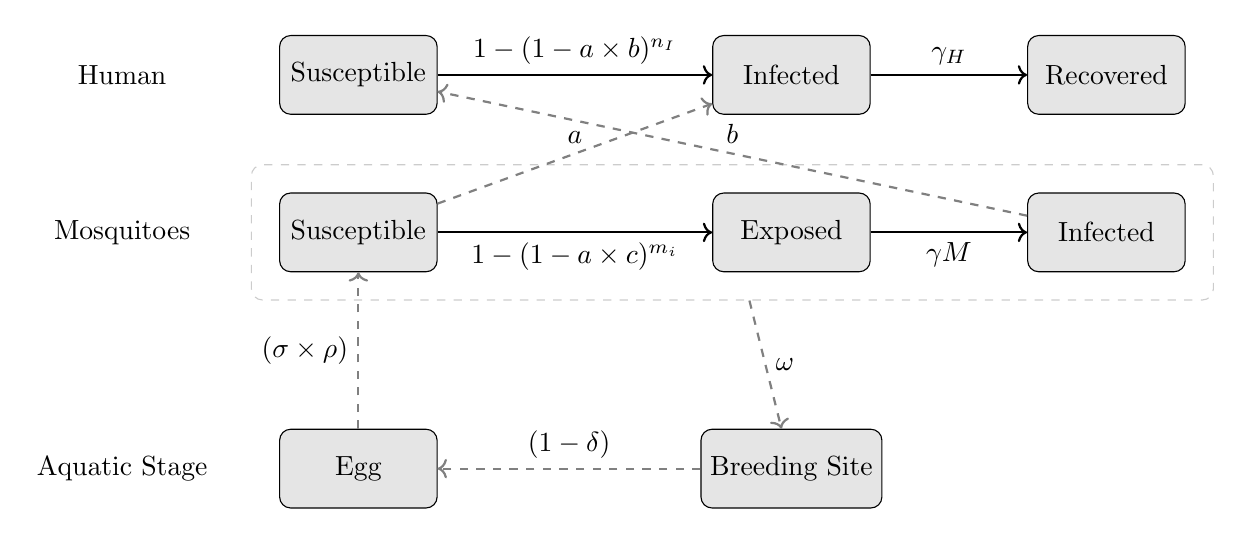
\begin{tikzpicture}[ node distance = 4.0cm, block/.style = {rectangle, draw,
					minimum width=2cm, minimum height=1cm, fill=lightgray, rounded corners,
					fill opacity=0.4, text=black, text opacity=1.0}, arrow/.style = {->,
					thick}, dashedarrow/.style = {->, thick, dashed}, dashedbox/.style =
				{draw, dashed, inner sep=10pt, rounded corners, opacity=0.2}
			% Define dashed box style
		]

		% Nodes
		\node (P) {Human}; \node [block, right of=P, xshift=-1cm] (S)
		{Susceptible}; \node [block, right of=S, xshift=1.5cm] (I) {Infected};
		\node [block, right of=I] (R) {Recovered};
		% \node[dashedbox, fit=(S) (I) (R)] (Box) {};

		% Arrows
		\draw [arrow] (S) -- (I) node[midway, above, color=black] {$1 - (1 - a
				\times b)^{n_{I}}$}; \draw [arrow] (I) -- (R) node[midway, above,
			color=black] {$\gamma_H$};

		\node [below of=P, yshift=2cm] (M) {Mosquitoes}; \node [block, right
			of=M, below of=P, yshift=2cm, xshift=-1cm] (SM) {Susceptible}; \node
		[block, right of=SM, below of=S, yshift=2cm, xshift=1.5cm] (EM)
		{Exposed}; \node [block, right of=EM, below of=I, yshift=2cm] (IM)
		{Infected};

		\node[dashedbox, fit=(SM) (EM) (IM)] (Box2) {};

		% Arrows
		\draw [arrow] (SM) -- (EM) node[midway, below, color=black] {$1 - (1 - a
				\times c)^{m_i}$}; \draw [arrow] (EM) -- (IM) node[midway, below,
			color=black] {$\gamma M$};

		\draw [dashedarrow, color=gray] (SM) -- (I) node[midway, above,
			color=black] {$a$}; \draw [dashedarrow, color=gray] (IM) -  - (S)
		node[midway, above, color=black] {$b$};

		%
		\node [below of=M, yshift=1cm] (AQ) {Aquatic Stage}; \node [block, right
			of=B, below of=M, yshift=1cm, xshift=-1cm] (EGG) {Egg};

		\node [block, right of=EGG, below of=SM, yshift=1cm, xshift=1.5cm] (BS)
		{Breeding Site};

		\draw [dashedarrow, color=gray] (Box2) -- (BS) node[midway, right,
			color=black] {$\omega$};

		\draw [dashedarrow, color=gray] (BS) -- (EGG) node[midway, above,
			color=black] {$(1 - \delta)$};

		\draw [dashedarrow, color=gray] (EGG) -- (SM) node[midway, left,
			color=black] {$(\sigma \times \rho)$};

		%
		% \node [below of=AQ, yshift=1cm] (BS) {Breeding Site:}; \node [block,
		% right of=BS, below of=EGG, yshift=1cm] (EGG) {Egg};
	\end{tikzpicture}

	\caption{Simplified agent interaction flowchart.}
	\label{fig:simplified-agent-interaction}
\end{figure}


\begin{itemize}
	\item \textbf{Human Agent:}
	      \begin{itemize}
		      \item \textbf{Location}: For each human, two blocks are randomly defined to
		            represent work and resting places. The exact point inside of each block is
		            also defined randomly.
		      \item \textbf{Move}: Considering the basic people's routines, they cycle
		            every day between two locations. It is assumed that humans have a residence
		            and a destination point, which may be, for example, school or work. The
		            movement is based on daily hours; each human has a ``$start\_work\_time$"
		            that is a time between 5 AM and 8 AM, indicating the time when the agent
		            starts to move from home to its destination, setting the current objective
		            to ``working". The ``$end\_work\_time$" follows the same pattern,
		            representing the return home between 4 PM and 7 PM, changing the current
		            objective to ``resting''.
		      \item \textbf{Change to Infected state}: Changing a human agent from
		            susceptible to infected requires interaction with infected mosquitoes. The
		            higher the number of infected mosquitoes nearby, the greater the chance of
		            this state transition. Assume $n_I$ as the number of infected mosquitoes
		            within a 1-meter distance and the probability of a human being infected by
		            the bite of an infected mosquito. From these values, consider $(a \times b)$
		            as the probability of a human becoming infected. Thus, the chance of
		            changing from a susceptible to an infected state is given by $1 - (1 - a
			            \times b)^{n_{I}}$.
		      \item  \textbf{Change to Recovered state}: Changing from infected to
		            recovered depends on the parameter $\gamma_H$.
	      \end{itemize}

	\item \textbf{Breeding Site Agent.}
	      \begin{itemize}
		      \item \textbf{Location}: Each breeding site is located at a random point
		            inside a street block.
		      \item \textbf{Create new eggs}: When a mosquito lays an egg at a breeding
		            site, this interaction creates a new Egg agent in the simulation. This new
		            egg is associated with the breeding site, and this decision impacts the
		            movement range of the adult mosquito.
	      \end{itemize}

	\item \textbf{Egg Agent.}
	      \begin{itemize}
		      \item \textbf{Location}: All Egg agents are located inside breeding sites.
		      \item \textbf{Change to  Adult phase}: The change from aquatic to adult
		            phase depends on the maturation rate ($\sigma$), and the successfully
		            hatched egg rate ($\rho$). The probability of an egg changing to the adult
		            stage is given by $\sigma \times \rho$.
		      \item \textbf{Aquatic Phase Death}: The death of an egg in the aquatic phase
		            depends on the mortality rate ($\delta$).
	      \end{itemize}

	\item \textbf{Mosquito Agent.}
	      \begin{itemize}
		      \item \textbf{Location}: Each mosquito is associated with a Breeding Site,
		            and its starting location is a random point inside a circle with a
		            $100$-meter radius, centered on the breeding site.
		      \item \textbf{Move}: Each mosquito has a $20\%$ chance of remaining
		            stationary during the cycle. If the agent decides to move, this action is
		            carried out randomly and at a random distance from the current location.
		            However, the destination is always close to the starting point, limited by a
		            radius of $100$ meters from the associated breeding site.
		      \item  \textbf{Oviposition}: The frequency and quantity of eggs that
		            mosquitoes lay depend on the number of breeding sites nearby (specifically,
		            within one meter of the current location), the oviposition rate ($\phi$),
		            and the biotic capacity of the mosquitoes ($\omega$). Each mosquito selects
		            a random breeding site, and based on $\phi$, the mosquitoes can lay a random
		            number of eggs ranging from $1$ to $\omega$.
		      \item \textbf{Change to Exposed state}: changing from susceptible to exposed
		            depends on the number of infected humans nearby. The larger this number, the
		            greater the chance of changing the state. Considering $a$ as the average
		            bite rate per day, $c$ as the probability of the mosquito being infected by
		            the virus, and $m_I$ as the number of infected people in the vicinity of the
		            mosquito, the probability of a mosquito changing from susceptible to
		            infected is given by $1 - (1 - a \times c)^{m_I}$.
		      \item \textbf{Change to  Infected state}: The transition from the exposed to
		            the infected state in mosquitoes is governed by the parameter $\gamma_M$.
		      \item \textbf{Die}: The death of the mosquitoes can occur during any state,
		            and the chance is given by the parameter $\mu_M$.
	      \end{itemize}
\end{itemize}

The flow of time in the simulation is based on cycles. Each cycle represents a
moment in time during which all agents perform their specific actions. In this
work, each cycle represents a time skip of 12 hours. Since the simulation runs
over real dates, the starting hour of the initial date of the simulation is
05:30 AM. This decision ensures that all cycles occur at 05:30 AM/PM, which are
moments of thermal inversions known as the most active time for mosquitoes. In
addition, these hours divide the human population into work and home locations.

The model implementation was developed in the GAMA
Platform\footnote{\url{https://gama-platform.org/}}~\citep{taillandier:2019}, a
tool designed specifically for \gls{mabs}. GAMA operates using a modeling
language called GAML (Gama Modeling Language), which is an agent-oriented
language. This means that everything active in the model can be represented in
GAMA as an agent. GAMA provides an interface to manipulate input/output data
from the simulation, which enables integration with other tools that interact
with the agents of the simulation. Figure~\ref{fig:example-gama} illustrates a
geospatial agent-based simulation of dengue transmission dynamics in
\textit{Alto Santo}, Brazil, modeled in the GAMA platform using \gls{osm} data.
Human populations are represented as yellow dots, red dots denote \textit{Aedes
	aegypti} mosquito population and black nodes are breeding sites. Potential
breeding sites are excluded from this visualization layer, as their simulated
locations are confined to street blocks. This simplification ensures visual
clarity while retaining the model’s focus on human-mosquito spatial
interactions.

\begin{figure}[!ht]
	\centering
	\includegraphics[width=16cm, height=10cm]{images/gama-example.png}
	\caption{Geographic view in GAMA platform.}
	\label{fig:example-gama}
\end{figure}

\section{Data Analysis}\label{sec:data-analysis}

\subsection{Limoeiro do Norte and Alto Santo Cities}\label{subsec:limoeiro-do-norte-and-alto-santo-cities}

This section presents a analysis of the notified cases from the cities of
\textit{Alto Santo} and \textit{Limoeiro do Norte} in the state of Ceará,
Brazil. These notifications are from 2015 to 2022, and they were obtained
through the city health departments through the
\gls{sinan}~\cite{laguardia:2004}. The data is organized in tables that contain
157 information fields from the medical service sheets. From \textit{Alto Santo}
city, we obtained 630 notifications in the data from 2016 to 2022.
\textit{Limoeiro do Norte} city has reported 3829 Dengue and 414 Chikungunya
cases from 2015 to 2021. The data from both cities gives a total of 4873 cases
reported in the \gls{sinan}.

According to the \gls{ibge}\footnote{\url{https://www.ibge.gov.br/}}, in the
last demographic census carried out in 2022, the \textit{Alto Santo} resident
population was 14,155 people. In \textit{Limoeiro}, this value increases to
59,560 residents, more than four times the population of \textit{Alto Santo}.
The urban area of \textit{Alto Santo} is only around 2 km$^2$, while
\textit{Limoeiro} has almost 15 km$^2$. The city centers extracted from the
\gls{osm} are presented in Figure~\ref{fig:osm-graph-examples}.

\begin{figure}[ht!]
	\begin{minipage}[c]{.5\textwidth}
		\includegraphics[width=7cm, height=6cm]{images/alto-santo-osm.png}
		\subcaption{Map of Alto Santo downtown.}
	\end{minipage}
	\begin{minipage}[c]{.5\textwidth}
		\includegraphics[width=7cm, height=6cm]{images/limoeiro-mapa.png}
		\subcaption{Map of Limoeiro downtown.}
	\end{minipage}
	\caption{\label{fig:osm-graph-examples} Maps extracted from \gls{osm}.}
\end{figure}

Figure~\ref{fig:cases-per-status} shows the number of notifications clustered by
the final classification for the complete \gls{sinan} dataset, including options
such as positive for Dengue or Chikungunya, Dengue with alarm signals, severe
Dengue, discarded cases, and cases pending closure. According to the current
health department of \textit{Alto Santo}, there was underreporting of cases in
the \gls{sinan} during the initial years. This can be observed, for example, in
Figure~\ref{fig:cases-per-year}, which presents the number of notifications
grouped by year for each city. In \textit{Alto Santo}, in 2017, more than 200
notifications remained pending.

\begin{center}
	\begin{figure}[ht!]
		\centering
		\includegraphics[width=8cm, height=7cm]{images/cases-per-status.pdf}
		\caption{Number of notifications considering both cities under
			study.}\label{fig:cases-per-status}
	\end{figure}
\end{center}

Analyzing the data presented in Figure~\ref{fig:cases-per-year}, except for 2018
in \textit{Limoeiro do Norte}, there are at least 150 positive cases each year,
with the highest number of cases occurring in 2019 and 2020. The year of 2020
was considered an epidemic year, reporting more than 1450 positive cases. In
\textit{Alto Santo}, more than half of the total notifications were reported
only in 2017, with more cases pending than confirmed positive or negative. The
number of positive notifications in all other years is lower than 75 and almost
no cases in the two years after 2017. According to conversations with the
\textit{Alto Santo} health department, except for 2017, none of the years were
characterized as epidemic seasons. The number of cases increased only in 2021.


\begin{center}
	\begin{figure}[ht!]
		\begin{minipage}[c]{.5\textwidth}
			\centering
			\includegraphics[width=6.5cm, height=7cm]{images/cases-per-year-Limoeiro do Norte.pdf}
			\subcaption{Notifications from Limoeiro.}
		\end{minipage}
		\begin{minipage}[c]{.5\textwidth}
			\centering
			\includegraphics[width=6.5cm, height=7cm]{images/cases-per-year-Alto Santo.pdf}
			\subcaption{Notifications from Alto Santo.}
		\end{minipage}
		\caption{\label{fig:cases-per-year} Number of notifications per year.}
	\end{figure}
\end{center}

Considering the total number of notifications and their distribution over the
years, it is evident that \textit{Limoeiro do Norte}, with a larger population,
also experiences a higher number of Dengue and Chikungunya cases every year. To
analyze the distribution of cases in the same granularity of time used by the
health departments, we selected the two years with the most notifications for
each city, specifically 2019/2020 for \textit{Limoeiro} and 2017/2021 for
\textit{Alto Santo} (Figures~\ref{fig:cases-per-week-limoeiro}
and~\ref{fig:cases-per-week-as}, respectively). These figures depict the
distribution of notifications for each \gls{ew} with at least one notification.

\begin{figure}[ht!]
	\begin{minipage}[c]{.9\textwidth}
		\centering
		\includegraphics[scale=0.32]{images/cases-per-week-2019-Limoeiro do Norte.pdf}
		\subcaption{Notifications from Limoeiro - 2019.}
	\end{minipage}
	\\
	\begin{minipage}[c]{.9\textwidth}
		\centering
		\includegraphics[scale=0.32]{images/cases-per-week-2020-Limoeiro do Norte.pdf}
		\subcaption{Notifications from Limoeiro - 2020.}
	\end{minipage}
	\caption{\label{fig:cases-per-week-limoeiro} Number of notifications per week
		- Limoeiro do Norte.}
\end{figure}

\begin{figure}[ht!]
	\begin{minipage}[c]{.9\textwidth}
		\centering
		\includegraphics[scale=0.32]{images/cases-per-week-2017-Alto Santo.pdf}
		\subcaption{Notifications from Alto Santo - 2017.}
	\end{minipage}
	\\
	\begin{minipage}[c]{.9\textwidth}
		\centering
		\includegraphics[scale=0.32]{images/cases-per-week-2021-Alto Santo.pdf}
		\subcaption{Notifications from Alto Santo - 2021.}
	\end{minipage}
	\caption{\label{fig:cases-per-week-as} Number of notifications per week - Alto
		Santo.}
\end{figure}


In \textit{Alto Santo}, during 2017, dengue cases were reported within the first
16 epidemiological weeks (\gls{ews}), peaking at 25 cases in week 4. Based on
the application, we can classify these notifications as either positive or
negative, given the high number of confirmed dengue cases during the same
period. In 2021, cases were recorded between \gls{ew} 14 and 48, with a lower
weekly incidence, reaching a peak of 9 confirmed cases in week 21.

From \textit{Limoeiro}, in 2019, cases are present in almost all weeks with
peaks of positive cases occurring between weeks 24 and 32, ranging from 10 to 29
cases. There is an epidemic season from weeks 20 to 38 of 2020, where the number
of cases is at least 40, and for 8 consecutive weeks after the 27 \gls{ew}, the
number of cases ranges from 80 to 123.

Two points need to be highlighted to understand this dataset. First,
underreporting likely occurred as infected individuals may not have pursued
hospital care due to: \textit{(1)} Knowing Dengue is seasonal, individuals often
self-diagnose when experiencing common disease symptoms, \textit{(2)} adherence
to clinically recommended protocols without formal testing, or \textit{(3)} mild
symptoms that did not disrupt daily activities. Second, the absence of
spatiotemporal records on vector-control interventions (e.g., insecticide
campaigns and larval habitat removal) obscures their impact on mosquito
populations and localized transmission dynamics. These limitations collectively
contribute to the observed fluctuations in notifications.

In both cities, public health strategies lack integration with digital
surveillance tools or predictive systems. Unfortunately, they rely on reactive
containment measures initiated only after spikes in confirmed dengue cases. This
firefighting approach - common across resource-constrained municipalities in
Brazil - fails to optimize prevention due to three key gaps: \textit{(i)}
delayed detection of epidemiological trends, \textit{(ii)} absence of
data-driven risk mapping to prioritize high-risk zones, and \textit{(iii)} ad
hoc resource allocation that overlooks transmission dynamics. Consequently,
interventions often occur too late to curb outbreaks effectively, perpetuating
cycles of suboptimal public health outcomes.



\section{Statistical Analysis of Results}\label{subsec:statistical-analysis}

\section{Instance Generation}\label{sec:instance-generation}

To identify (label) each city block, we employ a graph-theoretical procedure
that corresponds to finding the faces of a planar
embedding~\citep{diestel2024graph}. A planar embedding, also called a rotation
system, is defined for a planar graph by assigning, for each vertex $( i \in V
	)$, a cyclic ordering $C(i)$ of its neighbors (typically in clockwise order).
Intuitively, this defines the clockwise order of streets around each
intersection. This rotation system can be computed using the geometric slope of
each incident arc~\citep{PhilipKleinShayMozes}. As an illustrative example,
consider the graph in \ref{fig:non_isolated_nodes}. Its planar embedding can be
described by the function $C$ as shown in Table~\ref{tabnew}.

\begin{figure}[ht!]
	\centering
	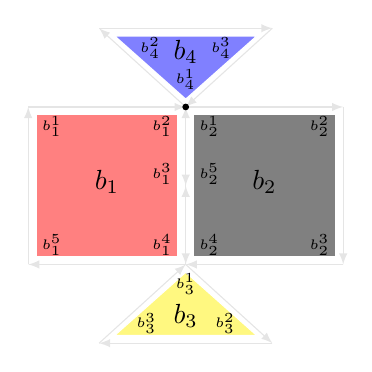
\begin{tikzpicture}[>=latex]
		% nodes
		% block A
		\coordinate (A1) at (0.1, 2.9);
		\coordinate (A2) at (1.9, 2.9);
		\coordinate (A3) at (1.9, 2);
		\coordinate (A4) at (1.9, 1.1);
		\coordinate (A5) at (0.1, 1.1);
		\coordinate (BorderA1) at (0, 3);
		\coordinate (BorderA2) at (2, 3);
		\coordinate (BorderA3) at (2, 2);
		\coordinate (BorderA4) at (2, 1);
		\coordinate (BorderA5) at (0, 1);
		% block B
		\coordinate (B1) at (2.1, 2.9);
		\coordinate (B2) at (3.9, 2.9);
		\coordinate (B3) at (3.9, 1.1);
		\coordinate (B4) at (2.1, 1.1);
		\coordinate (B5) at (2.1, 2);
		\coordinate (BorderB1) at (2, 3);
		\coordinate (BorderB2) at (4, 3);
		\coordinate (BorderB3) at (4, 1);
		\coordinate (BorderB4) at (2, 1);
		\coordinate (BorderB5) at (2, 2);
		% block C
		\coordinate (C1) at (2, 0.9);
		\coordinate (C2) at (2.9, 0.1);
		\coordinate (C3) at (1.1, 0.1);
		\coordinate (BorderC1) at (2, 1);
		\coordinate (BorderC2) at (3.1, 0);
		\coordinate (BorderC3) at (0.9, 0);
		% block B
		\coordinate (D1) at (2, 3.1);
		\coordinate (D2) at (1.1, 3.9);
		\coordinate (D3) at (2.9, 3.9);
		\coordinate (BorderD1) at (2, 3);
		\coordinate (BorderD2) at (0.9, 4);
		\coordinate (BorderD3) at (3.1, 4);
		% blocks
		\def\blockA{A1, A2, A3, A4, A5}
		\def\blockB{B1, B2, B3, B4, B5}
		\def\blockC{C1, C2, C3}
		\def\blockD{D1, D2, D3}
		% arcs
		\def\arcs{%
			% block A
			BorderA1 BorderA2
			BorderA2 BorderA3
			BorderA3 BorderA4
			BorderA4 BorderA5
			BorderA5 BorderA1
			% block B
			BorderB1 BorderB2
			BorderB2 BorderB3
			BorderB3 BorderB4
			BorderB4 BorderB5
			BorderB5 BorderB1
			% block C
			BorderC1 BorderC2
			BorderC2 BorderC3
			BorderC3 BorderC1
			% block D
			BorderD1 BorderD2
			BorderD2 BorderD3
			BorderD3 BorderD1
		}
		\readarray\arcs\Arcs[16,2]
		% print arcs
		\drawArcs{\Arcs}{\ArcsROWS}{->, gray!20, to path={-| (\tikztotarget)}}
		%block A
		\drawBlock{A1}{\blockA}{red!50};
		%block B
		\drawBlock{B1}{\blockB}{black!50};
		%block C
		\drawBlock{C1}{\blockC}{yellow!50};
		%block D
		\drawBlock{D1}{\blockD}{blue!50};
		% dot
		\filldraw[black] (BorderD1) circle (1pt);
		% blocks labels
		% A
		\node[xshift=2mm, yshift=-1.5mm] at (0.8, 2.2) {$b_1$};
		\node[xshift=2mm, yshift=-1.5mm] at (A1) {\tiny$b_1^1$};
		\node[xshift=-2mm, yshift=-1.5mm] at (A2) {\tiny$b_1^2$};
		\node[xshift=-2mm, yshift=1.5mm] at (A3) {\tiny$b_1^3$};
		\node[xshift=-2mm, yshift=1.5mm] at (A4) {\tiny$b_1^4$};
		\node[xshift=2mm, yshift=1.5mm] at (A5) {\tiny$b_1^5$};
		% B
		\node[xshift=2mm, yshift=-1.5mm] at (2.8, 2.2) {$b_2$};
		\node[xshift=2mm, yshift=-1.5mm] at (B1) {\tiny$b_2^1$};
		\node[xshift=-2mm, yshift=-1.5mm] at (B2) {\tiny$b_2^2$};
		\node[xshift=-2mm, yshift=1.5mm] at (B3) {\tiny$b_2^3$};
		\node[xshift=2mm, yshift=1.5mm] at (B4) {\tiny$b_2^4$};
		\node[xshift=2mm, yshift=1.5mm] at (B5) {\tiny$b_2^5$};
		% C
		\node[xshift=2mm, yshift=-1.5mm] at (1.8, 0.5) {$b_3$};
		\node[yshift=-1.5mm] at (C1) {\tiny$b_3^1$};
		\node[xshift=-4mm, yshift=1.5mm] at (C2) {\tiny$b_3^2$};
		\node[xshift=4mm, yshift=1.5mm] at (C3) {\tiny$b_3^3$};
		% B
		\node[xshift=2mm, yshift=-1.5mm] at (1.8, 3.85) {$b_4$};
		\node[yshift=2.5mm] at (D1) {\tiny$b_4^1$};
		\node[xshift=4.5mm, yshift=-1.5mm] at (D2) {\tiny$b_4^2$};
		\node[xshift=-4.5mm, yshift=-1.5mm] at (D3) {\tiny$b_4^3$};
	\end{tikzpicture}
	\caption{Example of non-isolated street-blocks.}
	\label{fig:non_isolated_nodes}
\end{figure}


\begin{table}[h!]
	\centering
	\caption{Connections for each city block}\label{tabnew}
	\begin{tabular}{cl}
		\hline
		\textbf{City Block} & \textbf{Connections}                      \\ \hline
		\( C(b^1_1) \)      & \( (b^5_1, b^2_1) \)                      \\
		\( C(b^2_1) \)      & \( (b^3_1, b^1_1, b^2_4, b^3_4, b^2_2) \) \\
		\( C(b^3_1) \)      & \( (b^4_1, b^1_2) \)                      \\
		\( C(b^4_1) \)      & \( (b^3_3, b^5_1, b^5_2, b^3_2, b^2_3) \) \\
		\( C(b^5_1) \)      & \( (b^1_1, b^4_1) \)                      \\
		\( C(b^2_2) \)      & \( (b^1_2, b^3_2) \)                      \\
		\( C(b^3_2) \)      & \( (b^4_2, b^2_2) \)                      \\
		\( C(b^2_3) \)      & \( (b^3_3, b^1_3) \)                      \\
		\( C(b^3_3) \)      & \( (b^1_3, b^2_3) \)                      \\
		\( C(b^2_4) \)      & \( (b^3_4, b^1_4) \)                      \\
		\( C(b^3_4) \)      & \( (b^1_4, b^2_4) \)                      \\ \hline
	\end{tabular}
\end{table}

With combinatorial embedding \( C \) and arc set \( A \), we identify all
bounded and unbounded faces of the planar graph using a traversal procedure
formalized in Algorithm~\ref{alg:find_faces}. Each face corresponds to a cyclic
sequence of arcs that form the boundary of a region enclosed by streets (i.e., a
city block). The algorithm iteratively traverses unused arcs in the graph by
following the clockwise ordering defined by \( C \), marking each arc as visited
once it has been assigned to a face. Each traversal terminates upon returning to
the starting arc, thus completing a cycle (face). This procedure ensures that
every face is uniquely defined by a sequence of arcs traversed in the clockwise
direction relative to the embedding. We note that every planar embedding has one
unbounded `outer' face encircling the whole graph. This outer face does not
correspond to any physical city block, so we exclude it from the set of labeled
blocks.


\begin{algorithm}[h!]
	\caption{Face-finding algorithm for planar embedding}
	\label{alg:find_faces}
	\begin{algorithmic}[1]
		\REQUIRE Planar graph \( D = (V, A) \), combinatorial embedding \( C \)
		\ENSURE Set of directed cycles \( \mathcal{F} \) representing faces

		\STATE Initialize \( \mathcal{F} \gets \emptyset \), and mark all arcs in \( A \) as unvisited
		\FOR{each unvisited arc \( a = (u, v) \in A \)}
		\STATE Set \( a_0 \gets a \), and mark \( a \) as visited
		\REPEAT
		\STATE Append \( a \) to \( f \)
		\STATE Let \( w \) be the next vertex after \( u \) in \( C(v) \) (i.e., clockwise successor of \( u \))
		\STATE Set \( a \gets (v, w) \); mark \( a \) as visited
		\STATE Update \( u \gets v \), \( v \gets w \)
		\UNTIL{\( a = a_0 \)}
		\STATE Add \( f \) to \( \mathcal{F} \)
		\ENDFOR
		\RETURN \( \mathcal{F} \)
	\end{algorithmic}
\end{algorithm}

\subsection{Real-case instances}\label{subsec:real_instances}

We collected real-world dengue notification data from 2015 to 2021 through the
municipal health departments of Alto Santo and Limoeiro do Norte, located in the
state of Ceará, Brazil. The data were extracted from the
\gls{sinan}~\cite{laguardia:2004}. During this period, Alto Santo reported 582
cases (2016-2021), and Limoeiro do Norte reported 4,243 cases (2015-2021),
totaling 4,825 confirmed dengue cases between the two cities. Our computational
benchmark consists of 39 instances based on these notifications. The addresses
of reported cases were geolocated using the OSMnx library~\cite{boeing:2017},
which provided latitude and longitude coordinates. Each case was mapped to its
corresponding city block, allowing us to integrate the case data with the street
network. Figure~\ref{fig:graph-examples} illustrates both the geographic maps and the
corresponding graph models of Alto Santo and Limoeiro do Norte, as derived from \gls{osm}. Figure~\ref{tab:real-instances} summarizes the key characteristics
of the benchmark used in the experimental evaluation.

\begin{figure}[h!]
	\begin{minipage}[c]{.49\textwidth}
		\centering
		\subfloat[Map of Alto Santo from OSM.]{\label{fig:altosanto}\includegraphics[width=7cm, height=6cm]{images/alto-santo-osm.png}}
	\end{minipage}%
	\begin{minipage}[c]{.49\textwidth}
		\centering
		\subfloat[Map of Limoeiro do Norte from OSM.]{\label{fig:limoeiro}\includegraphics[width=7cm, height=6cm]{images/limoeiro-osm.png}}
	\end{minipage}\\[2mm]
	\begin{minipage}[c]{.49\textwidth}
		\centering
		\subfloat[Graph of Alto Santo.]{\label{fig:Galtosanto}\includegraphics[width=7cm, height=6cm]{images/graph-alto-santo.png}}
	\end{minipage}%
	\begin{minipage}[c]{.49\textwidth}
		\centering
		\subfloat[Graph of Limoeiro do Norte.]{\label{fig:Glimoeiro}\includegraphics[width=7cm, height=6cm]{images/graph-limoeiro.png}}
	\end{minipage}
	\caption{\label{fig:graph-examples} Representation of the two cities used in the benchmark.}
\end{figure}


\begin{table}[h!]
	\centering
	\caption{Benchmark main characteristics.}
	\label{tab:real-instances}
	\begin{tabular}{lrrrrr}
		\hline
		\multicolumn{1}{c}{Instances}                                                &
		\multicolumn{1}{c}{$|V|$}                                                    &
		\multicolumn{1}{c}{$|A|$}                                                    &
		\multicolumn{1}{c}{$|B|$}                                                    &
		\multicolumn{1}{c}{\begin{tabular}[c]{@{}c@{}}Notified\\ Cases\end{tabular}} &
		\multicolumn{1}{c}{\begin{tabular}[c]{@{}c@{}}Blocks with\\ Cases (\%)\end{tabular}}                            \\ \hline
		AS-1000-2016                                                                 & 179  & 499  & 73  & 35   & 13.70 \\
		AS-1000-2017                                                                 & 179  & 499  & 73  & 194  & 36.99 \\
		AS-1000-2018                                                                 & 179  & 499  & 73  & 196  & 36.99 \\
		AS-1000-2019                                                                 & 179  & 499  & 73  & 196  & 36.99 \\
		AS-1000-2020                                                                 & 179  & 499  & 73  & 204  & 36.99 \\
		AS-1000-2021                                                                 & 179  & 499  & 73  & 218  & 36.99 \\ \hline
		AS-2000-2016                                                                 & 253  & 684  & 88  & 26   & 9.09  \\
		AS-2000-2017                                                                 & 253  & 684  & 88  & 174  & 29.55 \\
		AS-2000-2018                                                                 & 253  & 684  & 88  & 174  & 29.55 \\
		AS-2000-2019                                                                 & 253  & 684  & 88  & 174  & 29.55 \\
		AS-2000-2020                                                                 & 253  & 684  & 88  & 181  & 29.55 \\
		AS-2000-2021                                                                 & 253  & 684  & 88  & 195  & 30.68 \\ \hline
		AS-3000-2016                                                                 & 353  & 946  & 114 & 33   & 8.77  \\
		AS-3000-2017                                                                 & 353  & 946  & 114 & 198  & 24.56 \\
		AS-3000-2018                                                                 & 353  & 946  & 114 & 198  & 24.56 \\
		AS-3000-2019                                                                 & 353  & 946  & 114 & 198  & 24.56 \\
		AS-3000-2020                                                                 & 353  & 946  & 114 & 206  & 24.56 \\
		AS-3000-2021                                                                 & 353  & 946  & 114 & 225  & 24.56 \\ \hline
		LN-1000-2015                                                                 & 372  & 1063 & 152 & 18   & 7.89  \\
		LN-1000-2016                                                                 & 372  & 1063 & 152 & 26   & 10.53 \\
		LN-1000-2017                                                                 & 372  & 1063 & 152 & 50   & 17.11 \\
		LN-1000-2018                                                                 & 372  & 1063 & 152 & 51   & 17.11 \\
		LN-1000-2019                                                                 & 372  & 1063 & 152 & 66   & 20.39 \\
		LN-1000-2020                                                                 & 372  & 1063 & 152 & 163  & 29.61 \\
		LN-1000-2021                                                                 & 372  & 1063 & 152 & 168  & 31.58 \\ \hline
		LN-2000-2015                                                                 & 980  & 2866 & 443 & 174  & 6.77  \\
		LN-2000-2016                                                                 & 980  & 2866 & 443 & 337  & 9.03  \\
		LN-2000-2017                                                                 & 980  & 2866 & 443 & 527  & 12.19 \\
		LN-2000-2018                                                                 & 980  & 2866 & 443 & 543  & 12.64 \\
		LN-2000-2019                                                                 & 980  & 2866 & 443 & 875  & 14.22 \\
		LN-2000-2020                                                                 & 980  & 2866 & 443 & 2183 & 20.99 \\
		LN-2000-2021                                                                 & 980  & 2866 & 443 & 2316 & 21.67 \\ \hline
		LN-3000-2015                                                                 & 1212 & 3497 & 517 & 169  & 5.22  \\
		LN-3000-2016                                                                 & 1212 & 3497 & 517 & 336  & 7.54  \\
		LN-3000-2017                                                                 & 1212 & 3497 & 517 & 519  & 10.83 \\
		LN-3000-2018                                                                 & 1212 & 3497 & 517 & 533  & 11.03 \\
		LN-3000-2019                                                                 & 1212 & 3497 & 517 & 860  & 12.38 \\
		LN-3000-2020                                                                 & 1212 & 3497 & 517 & 2176 & 18.96 \\
		LN-3000-2021                                                                 & 1212 & 3497 & 517 & 2315 & 19.92 \\ \hline
	\end{tabular}%
\end{table}




\chapter{Computational Experiments}\label{chp:computational-experiments}

\section{Multi-Agent-Based Simulation}\label{sec:multi-agent-based-simulation}

This section presents the results obtained from the \gls{mabs} described in
Section~\ref{sec:mabs-dengue-virus}. The implementation uses GAMA Platform
version 1.9.2, the OSMnx Python Library~\cite{boeing:2017} 1.9.3 was used to
extract the map from \gls{osm}, and the street blocks are computed using the
procedure described in Section~\ref{sec:city-block-labeling}. The code is
available in this public repository on
Github\footnote{\url{https://github.com/cvaraujo/dengue-cbrp-mabs}}.

This study explores different combinations of parameters from
Table~\ref{tab:initial-pop-params} to identify the optimal configuration for
each city based on the average number (min and max) of cases per week in
multiple simulation runs. The precision and reliability of the results are
assessed through the Pearson correlation coefficient ($r$), \gls{mae}, and the
analysis of the simulated endemic channel.

\begin{table}[ht!]
	\centering
	\caption{Parameters for the initial state of the simulation.}
	\label{tab:initial-pop-params}
	\resizebox{\textwidth}{!}{%
		\begin{tabular}{c|l|c}
			\toprule
			Parameter & Description                                                              & Value                  \\
			\midrule
			$p$       & Number of people per $m^2$                                               & 0.006 - 0.01           \\
			$H_b$     & Number of people in block b                                              & $p \times A_b$         \\
			$H_0$     & Starting size of human population                                        & $\sum_{b = 1}^{B} H_b$ \\
			$M_h$     & Number of mosquitoes per human                                           & 0.50 - 3.00            \\
			$M_b$     & Percent of infected mosquitoes in a block without notifications          & 0.05 - 0.30            \\
			$M_{b}^i$ & Percent of infected mosquitoes in a block with at least one notification & 0.40 - 0.90            \\
			$BS$      & Number of potential Breeding Sites                                       & 50 - 500               \\
			\bottomrule
		\end{tabular}%
	}
\end{table}

\subsection{Data Processing}\label{subsec:data-processing}

First, the objective is to establish the initial population size by computing
the $p$ values. This work calculates the area of each street block as a polygon
using the Shapely\footnote{\url{https://shapely.readthedocs.io/en/stable/}} and
Geopandas\footnote{\url{https://geopandas.org/en/stable/}} Python libraries with
data imported from \gls{osm}. Since the investigation in this work focuses
mainly on urban areas, and both cities have vast territorial extensions that are
predominantly composed of rural areas, their overall population densities
reported in \gls{ibge} are low. For this reason, this work restricts the area
considered in the population density calculation to the city center and strictly
adjacent zones. However, there are no population data available at the level of
blocks or neighborhoods, and alternative sources were needed to improve the
values that estimate the resident population in the cities and then define the
initial population parameters for the simulation.

The choice of using a parameter ($p$) defined as persons per square meter
(m\textsuperscript{2}) ensures a good level of generalization for the
simulation, as the presence of this value allows the population to remain
proportionally adjusted for different experiments changing the size of the city
map. This can be particularly useful, for example, if we wish to simulate the
evolution of dengue cases in a single neighborhood.

Based on data provided by \gls{osm}, the urban area considered in Alto Santo
covers approximately 0.9~km\textsuperscript{2}, with an estimated population of
9,000 people living in the city centers. This yields a population density of $p
	= 0.01$ people per m\textsuperscript{2}. For Limoeiro, the approximate urban
area has 6~km\textsuperscript{2} and a population of 36000, which corresponds to
a value of \( p = 0.006 \) people per m\textsuperscript{2}. Since this
\gls{mabs} positions the individuals within blocks, the starting human
population consists of the sum of $p$ multiplied by the area of the
corresponding block. For Alto Santo, using a radius of 700~m inside OSMnx, 73
street blocks are generated and the starting human population is $H_0 = 5688$.
In Limoeiro, with a large urban area, the radius of 2000~m provides 563 blocks
and an initial population $H_0 = 29914$.

The starting size of the mosquito population is determined by $m = H_b \times
	M_h$, where the number of infected mosquitoes in the block is $M_b \times m$ for
blocks without cases and $M_b^{i} \times m$ otherwise. The starting number of
potential breeding sites is related to the parameter $BS$ and the blocks. For
each block, if there is at least one positive case, then there is at least one
breeding site. At the end of the initial scenario creation, if the breeding
sites located are fewer than $BS$, then the remaining were placed in random
blocks.

The \gls{mabs} initialize using epidemiological data from a specified start
date, incorporating historical notifications from the preceding week as
confirmed cases within the simulation blocks. This methodology is in line with
standard public health surveillance practices. To validate accuracy and quality,
the simulated case projections are systematically compared with actual weekly
reported cases over a 90-day evaluation period (equivalent to 180 simulation
cycles after initialization). The selected starting dates are selected based on
epidemiological periods within a reasonable number of notifications, as explored
in Section~\ref{sec:real-notifications}.

The parameters tested were $M_h = [0.5, 1, 2, 3]$, $M_b = [0.05, 0.1, 0.15, 0.2,
	0.3]$, $M_b^{i} = [0.4, 0.5, 0.6, 0.7, 0.8]$, and $BS = [50, 100, 200, 300,
	500]$. The analysis aggregates the results of 100 independent simulation trials
for each parameter configuration and start date, ensuring statistical robustness
in assessing model performance. The default maps of Alto Santo and Limoeiro
consider OSMnx radius of 700~m and 2000~m, respectively.

An independent set of initial dates was defined for each city. The objective of
the parameter exploration is to determine the best configuration based on
similarity with historical real-world data, which were mapped to the same map
segment used in the simulation. One set of parameters is considered better than
another using the number of ``wins'' for the dates on which these three
criteria, in the following order of precedence, were better: (1) higher
correlation between the simulated mean and the real data; (2) lower \gls{mae}
between the simulated mean and the historical data; (3) number of weeks in which
the real case notifications fall within the Simulation Endemic Channel, i.e.,
the range between the highest and lowest number of simulated cases in a given
week. The concept of endemic channel is used by public health departments to
assess how the number of cases in the current \gls{ew} compares with the
historical in previous years.


\subsection{Results for Alto Santo}

To determine the start dates for the experiments, we selected the two years with
the highest number of positive or pending notifications (2017 and 2021). The
cases were then grouped by epidemiological week, as shown in
Figure~\ref{fig:cases-per-week-as}. The objective is to focus on periods with
the highest number of cases and consistency between adjacent weeks, while
avoiding intervals with few or no cases. The experiments explore different
starting dates within these periods to analyze the simulation's behavior when
initiated at distinct moments along the endemic curve. Only historical
notifications that can be assigned to a block in the simulation are considered,
ensuring a fair comparison.

For better visualization of the results achieved by the simulator,
Figure~\ref{fig:avg-result-2017-01-as} presents the results for the best
configuration considering the following starting dates: \textit{(1)}~2017-01-08,
\textit{(2)}~2017-01-15, \textit{(3)}~2017-01-22, \textit{(4)}~2017-01-29,
\textit{(5)}~2021-05-30, and \textit{(6)}~2021-06-06. The X-axis represents the
week number, the Y-axis represents the number of cases, the solid black line
represents the total real notifications in the week, the dashed line represents
the average number of cases across simulations with the same starting scenario,
and the light gray ``$\times$'' markers represent the number of cases for a
given simulation run.

\begin{figure}[!ht]
	\begin{minipage}[c]{.45\textwidth}
		\centering
		\includegraphics[scale=0.4]{images/experiments-as/AS-2017-01-08.pdf}
		\subcaption{\label{subfig:as-a} 2017-01-08}
	\end{minipage}
	\hspace{0.5cm}
	\begin{minipage}[c]{.45\textwidth}
		\centering
		\includegraphics[scale=0.4]{images/experiments-as/AS-2017-01-15.pdf}
		\subcaption{\label{subfig:as-b} 2017-01-15}
	\end{minipage}
	\\
	\begin{minipage}[c]{.45\textwidth}
		\centering
		\includegraphics[scale=0.4]{images/experiments-as/AS-2017-01-22.pdf}
		\subcaption{\label{subfig:as-c} 2017-01-22}
	\end{minipage}
	\hspace{0.5cm}
	\begin{minipage}[c]{.45\textwidth}
		\centering
		\includegraphics[scale=0.4]{images/experiments-as/AS-2017-01-29.pdf}
		\subcaption{\label{subfig:as-d} 2017-01-29}
	\end{minipage}
	\\
	\begin{minipage}[c]{.45\textwidth}
		\centering
		\includegraphics[scale=0.4]{images/experiments-as/AS-2021-05-30.pdf}
		\subcaption{\label{subfig:as-e} 2021-05-30}
	\end{minipage}
	\hspace{0.5cm}
	\begin{minipage}[c]{.45\textwidth}
		\centering
		\includegraphics[scale=0.4]{images/experiments-as/AS-2021-06-06.pdf}
		\subcaption{\label{subfig:as-f} 2021-06-06}
	\end{minipage}
	\caption{\label{fig:avg-result-2017-01-as} Comparison of simulation and real cases from \textit{Alto Santo} for different starting dates.}
\end{figure}

The results represented in Figure~\ref{fig:avg-result-2017-01-as} correspond to
the variable parameters $M_h = 1$, $BS = 50$, $M_b = 0.05$ and $M_b^{i} = 0.4$,
which is the combination that achieved the best results considering the highest
correlation values ($r$) among all configurations for \textit{Alto Santo}. More
detailed information on these results is discussed later in this section.
%
Table~\ref{tab:statistical-data-as} shows the values of \gls{mae}, the
correlation of the average simulated cases with the real notification ($r$) and
the confidence interval (CI), in addition to the graphical results presented in
Figure~\ref{fig:avg-result-2017-01-as}.

\begin{table}[!ht]
	\centering
	\caption{Statistical values from the best configuration - \textit{Alto Santo} city.}
	\label{tab:statistical-data-as}
	\small{%
		\begin{tabular}{lrrrr}
			\toprule
			\multicolumn{1}{c}{\textbf{Date}}       &
			\multicolumn{1}{c}{\textbf{MAE}}        &
			\multicolumn{1}{c}{\textbf{$r$}}        &
			\multicolumn{1}{c}{\textbf{$CI_{min}$}} &
			\multicolumn{1}{c}{\textbf{$CI_{max}$}}                                      \\ \midrule
			2017-01-08                              & 5.67 & \textbf{0.83} & 0.61 & 0.94 \\
			2017-01-15                              & 5.20 & \textbf{0.93} & 0.82 & 0.97 \\
			2017-01-22                              & 8.40 & \textbf{0.90} & 0.75 & 0.96 \\
			2017-01-29                              & 2.80 & \textbf{0.92} & 0.80 & 0.97 \\
			2021-05-30                              & 0.94 & \textbf{0.84} & 0.62 & 0.94 \\
			2021-06-06                              & 1.92 & \textbf{0.77} & 0.49 & 0.91 \\ \bottomrule
		\end{tabular}%
	}
\end{table}

All experiments strongly correlate with real cases, achieving correlation
coefficients of at least $0.77$ with positive confidence intervals. This strong
correlation indicates that the average number of simulated cases per week
closely matches the real number of cases. The endemic channel generated in each
image of~\ref{fig:avg-result-2017-01-as} has a difference of at most 10 cases
from the real notifications when they are outside the endemic channel for a
given \gls{ew}, which represents a small deviation from reality.

\subsection{Results for Limoeiro}

The years 2019 and 2020 are selected for \textit{Limoeiro} city, and the number
of cases per week is shown in Figure~\ref{fig:cases-per-week-limoeiro}.
Figure~\ref{fig:avg-result-lim} presents the results for the following starting
dates: \textit{(1)}~2019-04-14, \textit{(2)}~2019-05-05,
\textit{(3)}~2020-06-21, \textit{(4)}~2020-07-05, \textit{(5)}~2020-07-19, and
\textit{(6)}~2020-07-26. Due to the extreme difference in the number of cases
between the two years for \textit{Limoeiro}, where 2020 has more than 1000
notifications than 2019, it was not possible to define a set of parameters that
fit well for both years with such different samples and behavior.
Figures~\ref{subfig:lim-a} and~\ref{subfig:lim-b} show the best results obtained
with the parameters $M_h = 0.5$, $BS = 100$, $M_b = 0.05$ and $M_b^{i} = 0.4$.
Figures~\ref{subfig:lim-c} to~\ref{subfig:lim-f} present the results with the
following parameters set $M_h = 1$, $BS = 500$, $M_b = 0.20$ and $M_b^{i} =
	0.9$.

\begin{figure}[!ht]
	\begin{minipage}[c]{.45\textwidth}
		\centering
		\includegraphics[scale=0.4]{images/experiments-lim/LIM-2019-04-14.pdf} \\
		\vspace{-0.3cm}
		\subcaption{\label{subfig:lim-a} 2019-04-14}
		% {\label{subfig:lim-a} 2019-04-14}
	\end{minipage}
	\hspace{0.5cm}
	\begin{minipage}[c]{.45\textwidth}
		\centering
		\includegraphics[scale=0.4]{images/experiments-lim/LIM-2019-05-05.pdf} \\
		\vspace{-0.3cm}
		\subcaption{\label{subfig:lim-b} 2019-05-05}
		% {\label{subfig:lim-b}\scriptsize (b) From 2019-05-05}
	\end{minipage}
	\\
	\begin{minipage}[c]{.45\textwidth}
		\centering
		\includegraphics[scale=0.4]{images/experiments-lim/LIM-2020-06-21.pdf} \\
		\vspace{-0.3cm}
		\subcaption{\label{subfig:lim-c} 2020-06-21}
		% {\label{subfig:lim-c}\scriptsize (c) From 2020-06-21}
	\end{minipage}
	\hspace{0.5cm}
	\begin{minipage}[c]{.45\textwidth}
		\centering
		\includegraphics[scale=0.4]{images/experiments-lim/LIM-2020-07-05.pdf} \\
		\vspace{-0.3cm}
		\subcaption{\label{subfig:lim-d} 2020-07-05}
		% {\label{subfig:lim-d}\scriptsize (d) From 2020-07-05}
	\end{minipage}
	\\
	\begin{minipage}[c]{.45\textwidth}
		\centering
		\includegraphics[scale=0.4]{images/experiments-lim/LIM-2020-07-19.pdf} \\
		\vspace{-0.3cm}
		\subcaption{\label{subfig:lim-e} 2020-07-19}
		% {\label{subfig:lim-e} \scriptsize (e) From 2020-07-19}
	\end{minipage}
	\hspace{0.5cm}
	\begin{minipage}[c]{.45\textwidth}
		\centering
		\includegraphics[scale=0.4]{images/experiments-lim/LIM-2020-07-26.pdf} \\
		\vspace{-0.3cm}
		\subcaption{\label{subfig:lim-f} 2020-07-26}
		% {\label{subfig:lim-f}\scriptsize (f) From 2020-07-26}
	\end{minipage}
	\caption{\label{fig:avg-result-lim} Comparison of simulation and real cases from \textit{Limoeiro} for different starting dates.}
\end{figure}

Table~\ref{tab:statistical-data-lim} shows the values of \gls{mae}, the correlation of the average simulated cases with the real notification ($r$), and the confidence interval of the results presented in Figures~\ref{fig:avg-result-lim}.

\begin{table}[!ht]
	\centering
	\caption{Statistical values from the best configuration - \textit{Limoeiro} city.}
	\label{tab:statistical-data-lim}
	\small{%
		\begin{tabular}{lrrrr}
			\toprule
			\multicolumn{1}{c}{\textbf{Date}}       &
			\multicolumn{1}{c}{\textbf{MAE}}        &
			\multicolumn{1}{c}{\textbf{$r$}}        &
			\multicolumn{1}{c}{\textbf{$CI_{min}$}} &
			\multicolumn{1}{c}{\textbf{$CI_{max}$}}                                        \\ \midrule
			2019-04-14                              & 2.99  & 0.06          & -0.41 & 0.51 \\
			2019-05-05                              & 3.28  & 0.09          & -0.38 & 0.53 \\
			2020-06-21                              & 27.97 & 0.30          & -0.18 & 0.67 \\
			2020-07-05                              & 13.90 & \textbf{0.76} & 0.45  & 0.90 \\
			2020-07-19                              & 4.49  & \textbf{0.97} & 0.93  & 0.99 \\
			2020-07-26                              & 9.27  & \textbf{0.96} & 0.90  & 0.99 \\ \bottomrule
		\end{tabular}%
	}
\end{table}

In 2019, the analysis of \textit{Limoeiro} City’s epidemiological data revealed
a weak correlation (values approaching zero), as indicated by the experimental
results. However, the associated \gls{mae} metrics were modest, ranging from
$2.99$ to $3.28$. Figures~\ref{subfig:lim-a} and~\ref{subfig:lim-b} illustrate
the weekly case distribution, highlighting irregular temporal patterns despite
the low overall incidence (with a peak of 12 notifications in the highest week).
In particular, only 4 of the 14 analyzed \gls{ew} exceeded the boundaries of the
simulated endemic channel.

Discrepancies between observed and expected case counts were predominantly minor
(1-2 cases), except for the $10^{th}$ and $13^{th}$ weeks, which each recorded
12 notifications and deviated by 9 cases from the channel’s upper limit. This
suggests that while the statistical correlation was weak, most of the weekly
case counts aligned with or remained close to the endemic channel. The results
show that even in low-incidence settings, localized fluctuations can occur
without systematically breaching expected epidemiological thresholds.

Figures~\ref{subfig:lim-c} and~\ref{subfig:lim-d} represent two simulations
started two weeks apart. In the first scenario, starting in 2020-06-21, the
model yields a weak correlation $(r = 0.3)$, as it anticipates a case peak in
the initial weeks, while the observed data show a delayed surge in the sixth
week. This temporal misalignment probably reflects limitations in model
calibration, including insufficient historical data and an inability to
integrate time-dependent variables that influence case trajectories.

In contrast, the second simulation, considering the start date of 2020-07-05 and
the initiation of the simulation two weeks later, shows a strong correlation ($r
	= 0.76$) with a positive confidence interval (CI), indicating a significantly
improved alignment with real-world trends. Here, the later start date probably
allowed the model to incorporate critical early phase data, enhancing its
predictive accuracy. These results highlight the sensitivity of epidemiological
models to initialization timing and the importance of adaptive calibration to
account for dynamic real-world factors.

Figures~\ref{subfig:lim-e}--\ref{subfig:lim-f}  demonstrate near-perfect
correlation coefficients ($r = 0.97$ and $r = 0.96$, respectively), reflecting
an exceptional alignment between simulated and observed case trends. These
simulations were initialized during peak cases in incidence periods for both
cities, the highest recorded in the notification dataset. The proximity of these
starting dates to the epidemiological peak likely allowed the model to capture
critical transmission dynamics, resulting in highly accurate projections. This
outcome confirms robustness when calibrated during periods of increased disease
activity, where the underlying patterns may be more pronounced and predictable.


\subsection{Simulation Quality Assessment}

Taking into account all the results presented, it is possible to highlight the
strengths of our \gls{mabs} that achieve good results for all simulations in
\textit{Alto Santo}. These outcomes present a strong correlation for all cases
and a good fit of the real data inside the simulated endemic channel. The
\gls{mabs} also presents a strong correlation for half of the simulations for
\textit{Limoeiro} and a good adjustment of the endemic channel to contain the
historical progression of notifications.

In some instances, the simulation's inability to accurately capture real-world
data may be attributed to unmodeled factors. For example, the model currently
does not account for the influence of climate, vector control efforts,
under-reporting, population density, and geographic features like vacant land
and proximity to water bodies. These factors can significantly impact disease
transmission dynamics, however, may not be fully represented in the current
simulation model.

Although the current \gls{mabs} framework cannot dynamically adapt parameters in
response to real-time data, it remains a robust analytical tool when combined
with the calibration of strategic parameters and domain expertise. By
integrating the principles of \gls{mabs} with epidemiological insights specific
to dengue transmission, researchers can identify optimal parameter
configurations that produce highly accurate simulations. Inclusion of real-time
data streams or detailed geographic information could further improve the
precision of the model. However, such enhancements are not prerequisites for
generating meaningful results.

Thus, it is possible to claim that the proposed \gls{mabs} is a reliable and
accurate simulation methodology, capable of generating scenarios that account
for both casual disease spread and endemic seasons in the cities of \textit{Alto
	Santo} and \textit{Limoeiro}, even with limitations in accurate and essential
information. The methodology can be further enhanced with additional data, and
the simplified programming language facilitates the integration of new features
and information into the \gls{mabs}. This approach can be used as a
visualization and decision support tool, primarily considering the generated
endemic channel and the fact that it is easy to simulate for other cities
assuming the existence of basic geographic information and historical data to
improve the best fit of the variable parameters.



\include{textual/6-conclusions}

% As referências:
\bibliographystyle{plain}
\bibliography{ic-tese-v3}


% Os anexos, se houver, vêm depois das referências:
% \appendix
% \chapter{Anexo 1}
% \chapter{Anexo 2}

\end{document}
